\documentclass[twoside]{book}

% Packages required by doxygen
\usepackage{fixltx2e}
\usepackage{calc}
\usepackage{doxygen}
\usepackage[export]{adjustbox} % also loads graphicx
\usepackage{graphicx}
\usepackage[utf8]{inputenc}
\usepackage{makeidx}
\usepackage{multicol}
\usepackage{multirow}
\PassOptionsToPackage{warn}{textcomp}
\usepackage{textcomp}
\usepackage[nointegrals]{wasysym}
\usepackage[table]{xcolor}

% NLS support packages
\usepackage[french]{babel}

% Font selection
\usepackage[T1]{fontenc}
\usepackage[scaled=.90]{helvet}
\usepackage{courier}
\usepackage{amssymb}
\usepackage{sectsty}
\renewcommand{\familydefault}{\sfdefault}
\allsectionsfont{%
  \fontseries{bc}\selectfont%
  \color{darkgray}%
}
\renewcommand{\DoxyLabelFont}{%
  \fontseries{bc}\selectfont%
  \color{darkgray}%
}
\newcommand{\+}{\discretionary{\mbox{\scriptsize$\hookleftarrow$}}{}{}}

% Page & text layout
\usepackage{geometry}
\geometry{%
  a4paper,%
  top=2.5cm,%
  bottom=2.5cm,%
  left=2.5cm,%
  right=2.5cm%
}
\tolerance=750
\hfuzz=15pt
\hbadness=750
\setlength{\emergencystretch}{15pt}
\setlength{\parindent}{0cm}
\setlength{\parskip}{3ex plus 2ex minus 2ex}
\makeatletter
\renewcommand{\paragraph}{%
  \@startsection{paragraph}{4}{0ex}{-1.0ex}{1.0ex}{%
    \normalfont\normalsize\bfseries\SS@parafont%
  }%
}
\renewcommand{\subparagraph}{%
  \@startsection{subparagraph}{5}{0ex}{-1.0ex}{1.0ex}{%
    \normalfont\normalsize\bfseries\SS@subparafont%
  }%
}
\makeatother

% Headers & footers
\usepackage{fancyhdr}
\pagestyle{fancyplain}
\fancyhead[LE]{\fancyplain{}{\bfseries\thepage}}
\fancyhead[CE]{\fancyplain{}{}}
\fancyhead[RE]{\fancyplain{}{\bfseries\leftmark}}
\fancyhead[LO]{\fancyplain{}{\bfseries\rightmark}}
\fancyhead[CO]{\fancyplain{}{}}
\fancyhead[RO]{\fancyplain{}{\bfseries\thepage}}
\fancyfoot[LE]{\fancyplain{}{}}
\fancyfoot[CE]{\fancyplain{}{}}
\fancyfoot[RE]{\fancyplain{}{\bfseries\scriptsize Généré par Doxygen }}
\fancyfoot[LO]{\fancyplain{}{\bfseries\scriptsize Généré par Doxygen }}
\fancyfoot[CO]{\fancyplain{}{}}
\fancyfoot[RO]{\fancyplain{}{}}
\renewcommand{\footrulewidth}{0.4pt}
\renewcommand{\chaptermark}[1]{%
  \markboth{#1}{}%
}
\renewcommand{\sectionmark}[1]{%
  \markright{\thesection\ #1}%
}

% Indices & bibliography
\usepackage{natbib}
\usepackage[titles]{tocloft}
\setcounter{tocdepth}{3}
\setcounter{secnumdepth}{5}
\makeindex

% Custom commands
\newcommand{\clearemptydoublepage}{%
  \newpage{\pagestyle{empty}\cleardoublepage}%
}

\usepackage{caption}
\captionsetup{labelsep=space,justification=centering,font={bf},singlelinecheck=off,skip=4pt,position=top}

%===== C O N T E N T S =====

\begin{document}

% Titlepage & ToC
\pagenumbering{alph}
\begin{titlepage}
\vspace*{7cm}
\begin{center}%
{\Large Paintbrush \\[1ex]\large 0.\+2 }\\
\vspace*{1cm}
{\large Généré par Doxygen 1.8.13}\\
\end{center}
\end{titlepage}
\clearemptydoublepage
\pagenumbering{roman}
\tableofcontents
\clearemptydoublepage
\pagenumbering{arabic}

%--- Begin generated contents ---
\chapter{Liste des choses à faire}
\label{todo}

\begin{DoxyRefList}
\item[\label{todo__todo000007}%
Global(e) \doxyref{create\+Player}{p.}{players_8h_a62a16a32a68ba4359f95213cd4e39e85} ()]Change the way to preconfigured players.  
\item[\label{todo__todo000003}%
Global(e) \doxyref{player\+:\+:dir}{p.}{structplayer_ac937d4dbbc71f2f0eb17958c8f6932bf} ]Make the direction totally vectorial on a circle  
\item[\label{todo__todo000002}%
Global(e) \doxyref{player\+:\+:scoreP}{p.}{structplayer_a260e160fd2a4cc082beb01802438dc13} ]Why double ? Long int isn\textquotesingle{}t sufficient ?  
\item[\label{todo__todo000005}%
Global(e) \doxyref{readline}{p.}{fonctions_8h_afe286242e48f523265fd5fcdae3f7358} (char $\ast$s, int n)]A way to describe the error ?  
\item[\label{todo__todo000001}%
Classe \doxyref{Screen}{p.}{struct_screen} ]Add the G\+UI zone  
\item[\label{todo__todo000004}%
Global(e) \doxyref{str\+\_\+replace}{p.}{fonctions_8h_afd361e8fd7c973935407a430d0c609a5} (char $\ast$$\ast$s, int token, int replacement)]Some validity tests for token and replacement. 
\end{DoxyRefList}
\chapter{Index des modules}
\section{Modules}
Liste de tous les modules \+:\begin{DoxyCompactList}
\item \contentsline{section}{Types de Bases}{\pageref{group___bases___types}}{}
\item \contentsline{section}{Types composites}{\pageref{group___composed___types}}{}
\end{DoxyCompactList}

\chapter{Index des structures de données}
\section{Structures de données}
Liste des structures de données avec une brève description \+:\begin{DoxyCompactList}
\item\contentsline{section}{\textbf{ Direction\+Vector} }{\pageref{struct_direction_vector}}{}
\item\contentsline{section}{\textbf{ Game\+Data} }{\pageref{struct_game_data}}{}
\item\contentsline{section}{\textbf{ painter} \\*Structure of a painter used everywhere }{\pageref{structpainter}}{}
\item\contentsline{section}{\textbf{ Player} \\*Structure of a \doxyref{Player}{p.}{struct_player} }{\pageref{struct_player}}{}
\item\contentsline{section}{\textbf{ player} }{\pageref{structplayer}}{}
\item\contentsline{section}{\textbf{ Screen} }{\pageref{struct_screen}}{}
\item\contentsline{section}{\textbf{ Speed\+Vector} }{\pageref{struct_speed_vector}}{}
\end{DoxyCompactList}

\chapter{Index des fichiers}
\section{Liste des fichiers}
Liste de tous les fichiers documentés avec une brève description \+:\begin{DoxyCompactList}
\item\contentsline{section}{\textbf{ defines.\+h} \\*Define all symbolic constants and some macros }{\pageref{defines_8h}}{}
\item\contentsline{section}{\textbf{ fonctions.\+c} \\*Implementation of some functions that can be used anywhere }{\pageref{fonctions_8c}}{}
\item\contentsline{section}{\textbf{ fonctions.\+h} \\*Define prototypes of common functions and includes other Headers files }{\pageref{fonctions_8h}}{}
\item\contentsline{section}{\textbf{ game\+\_\+fonctions.\+c} \\*Implement static and public core parts }{\pageref{game__fonctions_8c}}{}
\item\contentsline{section}{\textbf{ game\+\_\+fonctions.\+h} \\*Define the prototypes of core functions }{\pageref{game__fonctions_8h}}{}
\item\contentsline{section}{\textbf{ global\+\_\+inc.\+h} \\*Utility file for inclusion }{\pageref{global__inc_8h}}{}
\item\contentsline{section}{\textbf{ main.\+c} \\*Entry point of program }{\pageref{main_8c}}{}
\item\contentsline{section}{\textbf{ players.\+c} \\*Implement public players related functions and static painters related functions }{\pageref{players_8c}}{}
\item\contentsline{section}{\textbf{ players.\+h} \\*Define players related functions prototypes }{\pageref{players_8h}}{}
\item\contentsline{section}{\textbf{ quit.\+c} \\*Define functions used at exit }{\pageref{quit_8c}}{}
\item\contentsline{section}{\textbf{ quit.\+h} \\*Prototypes of exit functions }{\pageref{quit_8h}}{}
\item\contentsline{section}{\textbf{ types.\+h} \\*Types needed in program }{\pageref{types_8h}}{}
\end{DoxyCompactList}

\chapter{Documentation des modules}
\section{Types de Bases}
\label{group___bases___types}\index{Types de Bases@{Types de Bases}}
\subsection*{Structures de données}
\begin{DoxyCompactItemize}
\item 
struct \textbf{ Direction\+Vector}
\item 
struct \textbf{ Speed\+Vector}
\item 
struct \textbf{ Screen}
\end{DoxyCompactItemize}
\subsection*{Énumérations}
\begin{DoxyCompactItemize}
\item 
enum \textbf{ Direction} \{ \textbf{ D\+I\+R\+\_\+\+S\+T\+OP} =0, 
\textbf{ D\+I\+R\+\_\+\+A\+C\+T\+I\+VE} =1, 
\textbf{ D\+I\+R\+\_\+\+R\+E\+V\+E\+R\+SE} =-\/1
 \}
\item 
enum \textbf{ Brush\+Size} \{ \textbf{ B\+R\+U\+S\+H\+\_\+\+L\+I\+T\+T\+LE} =16, 
\textbf{ B\+R\+U\+S\+H\+\_\+\+N\+O\+R\+M\+AL} =32, 
\textbf{ B\+R\+U\+S\+H\+\_\+\+B\+IG} =64
 \}
\item 
enum \textbf{ Speed} \{ \textbf{ S\+P\+E\+E\+D\+\_\+\+N\+U\+LL} =0, 
\textbf{ S\+P\+E\+E\+D\+\_\+\+S\+L\+OW} =2, 
\textbf{ S\+P\+E\+E\+D\+\_\+\+A\+V\+E\+R\+A\+GE} =4, 
\textbf{ S\+P\+E\+E\+D\+\_\+\+F\+A\+ST} =6
 \}
\item 
enum \textbf{ Game\+State} \{ \textbf{ S\+T\+A\+T\+E\+\_\+\+Q\+U\+IT}, 
\textbf{ S\+T\+A\+T\+E\+\_\+\+P\+A\+U\+S\+ED}, 
\textbf{ S\+T\+A\+T\+E\+\_\+\+P\+L\+A\+Y\+I\+NG}, 
\textbf{ S\+T\+A\+T\+E\+\_\+\+C\+O\+N\+F\+I\+G\+U\+R\+A\+T\+I\+ON}
 \}
\item 
enum \textbf{ Control\+Keys} \{ \textbf{ C\+T\+R\+L\+\_\+\+K\+E\+Y\+\_\+\+R\+I\+G\+HT} =0, 
\textbf{ C\+T\+R\+L\+\_\+\+K\+E\+Y\+\_\+\+L\+E\+FT} =1, 
\textbf{ C\+T\+R\+L\+\_\+\+K\+E\+Y\+\_\+\+UP} =2, 
\textbf{ C\+T\+R\+L\+\_\+\+K\+E\+Y\+\_\+\+D\+O\+WN} =3
 \}
\end{DoxyCompactItemize}


\subsection{Description détaillée}


\subsection{Documentation du type de l\textquotesingle{}énumération}
\mbox{\label{group___bases___types_ga044b5d604dc46a25328861ae39e16a84}} 
\index{Types de Bases@{Types de Bases}!Brush\+Size@{Brush\+Size}}
\index{Brush\+Size@{Brush\+Size}!Types de Bases@{Types de Bases}}
\subsubsection{Brush\+Size}
{\footnotesize\ttfamily enum \textbf{ Brush\+Size}}



{\ttfamily \#include $<$\textbf{ types.\+h}$>$}

Enumeration of values related to the size of a Brush, for a painter. \begin{DoxyEnumFields}{Valeurs énumérées}
\raisebox{\heightof{T}}[0pt][0pt]{\index{B\+R\+U\+S\+H\+\_\+\+L\+I\+T\+T\+LE@{B\+R\+U\+S\+H\+\_\+\+L\+I\+T\+T\+LE}!Types de Bases@{Types de Bases}}\index{Types de Bases@{Types de Bases}!B\+R\+U\+S\+H\+\_\+\+L\+I\+T\+T\+LE@{B\+R\+U\+S\+H\+\_\+\+L\+I\+T\+T\+LE}}}\mbox{\label{group___bases___types_gga044b5d604dc46a25328861ae39e16a84aaa18849d3fba3457e62eea0e0730fe50}} 
B\+R\+U\+S\+H\+\_\+\+L\+I\+T\+T\+LE&Size of little painter (malus) \\
\hline

\raisebox{\heightof{T}}[0pt][0pt]{\index{B\+R\+U\+S\+H\+\_\+\+N\+O\+R\+M\+AL@{B\+R\+U\+S\+H\+\_\+\+N\+O\+R\+M\+AL}!Types de Bases@{Types de Bases}}\index{Types de Bases@{Types de Bases}!B\+R\+U\+S\+H\+\_\+\+N\+O\+R\+M\+AL@{B\+R\+U\+S\+H\+\_\+\+N\+O\+R\+M\+AL}}}\mbox{\label{group___bases___types_gga044b5d604dc46a25328861ae39e16a84a48bb202932d6bf0c818e4ed5e1a02bec}} 
B\+R\+U\+S\+H\+\_\+\+N\+O\+R\+M\+AL&Size of medium painter (normal) \\
\hline

\raisebox{\heightof{T}}[0pt][0pt]{\index{B\+R\+U\+S\+H\+\_\+\+B\+IG@{B\+R\+U\+S\+H\+\_\+\+B\+IG}!Types de Bases@{Types de Bases}}\index{Types de Bases@{Types de Bases}!B\+R\+U\+S\+H\+\_\+\+B\+IG@{B\+R\+U\+S\+H\+\_\+\+B\+IG}}}\mbox{\label{group___bases___types_gga044b5d604dc46a25328861ae39e16a84ae73ce3f81bfb92c2ec6368effaaf9a6f}} 
B\+R\+U\+S\+H\+\_\+\+B\+IG&Size of big painter (bonus) \\
\hline

\end{DoxyEnumFields}


Définition à la ligne 36 du fichier types.\+h.

\mbox{\label{group___bases___types_ga7c2c9ac31258225f5ea17a22c0118566}} 
\index{Types de Bases@{Types de Bases}!Control\+Keys@{Control\+Keys}}
\index{Control\+Keys@{Control\+Keys}!Types de Bases@{Types de Bases}}
\subsubsection{Control\+Keys}
{\footnotesize\ttfamily enum \textbf{ Control\+Keys}}



{\ttfamily \#include $<$\textbf{ types.\+h}$>$}

Indexes used for the Control\+Keys tabs. \begin{DoxyEnumFields}{Valeurs énumérées}
\raisebox{\heightof{T}}[0pt][0pt]{\index{C\+T\+R\+L\+\_\+\+K\+E\+Y\+\_\+\+R\+I\+G\+HT@{C\+T\+R\+L\+\_\+\+K\+E\+Y\+\_\+\+R\+I\+G\+HT}!Types de Bases@{Types de Bases}}\index{Types de Bases@{Types de Bases}!C\+T\+R\+L\+\_\+\+K\+E\+Y\+\_\+\+R\+I\+G\+HT@{C\+T\+R\+L\+\_\+\+K\+E\+Y\+\_\+\+R\+I\+G\+HT}}}\mbox{\label{group___bases___types_gga7c2c9ac31258225f5ea17a22c0118566a6e19dfe67c4de8c7715232088b48112a}} 
C\+T\+R\+L\+\_\+\+K\+E\+Y\+\_\+\+R\+I\+G\+HT&ID of R\+I\+G\+H\+T\+\_\+\+K\+EY \\
\hline

\raisebox{\heightof{T}}[0pt][0pt]{\index{C\+T\+R\+L\+\_\+\+K\+E\+Y\+\_\+\+L\+E\+FT@{C\+T\+R\+L\+\_\+\+K\+E\+Y\+\_\+\+L\+E\+FT}!Types de Bases@{Types de Bases}}\index{Types de Bases@{Types de Bases}!C\+T\+R\+L\+\_\+\+K\+E\+Y\+\_\+\+L\+E\+FT@{C\+T\+R\+L\+\_\+\+K\+E\+Y\+\_\+\+L\+E\+FT}}}\mbox{\label{group___bases___types_gga7c2c9ac31258225f5ea17a22c0118566a24ae796a5281ca0405b64e399f3b8d21}} 
C\+T\+R\+L\+\_\+\+K\+E\+Y\+\_\+\+L\+E\+FT&ID of L\+E\+F\+T\+\_\+\+K\+EY \\
\hline

\raisebox{\heightof{T}}[0pt][0pt]{\index{C\+T\+R\+L\+\_\+\+K\+E\+Y\+\_\+\+UP@{C\+T\+R\+L\+\_\+\+K\+E\+Y\+\_\+\+UP}!Types de Bases@{Types de Bases}}\index{Types de Bases@{Types de Bases}!C\+T\+R\+L\+\_\+\+K\+E\+Y\+\_\+\+UP@{C\+T\+R\+L\+\_\+\+K\+E\+Y\+\_\+\+UP}}}\mbox{\label{group___bases___types_gga7c2c9ac31258225f5ea17a22c0118566ae0ec38777f1a3af77313cbe3ac9edb55}} 
C\+T\+R\+L\+\_\+\+K\+E\+Y\+\_\+\+UP&ID of U\+P\+\_\+\+K\+EY \\
\hline

\raisebox{\heightof{T}}[0pt][0pt]{\index{C\+T\+R\+L\+\_\+\+K\+E\+Y\+\_\+\+D\+O\+WN@{C\+T\+R\+L\+\_\+\+K\+E\+Y\+\_\+\+D\+O\+WN}!Types de Bases@{Types de Bases}}\index{Types de Bases@{Types de Bases}!C\+T\+R\+L\+\_\+\+K\+E\+Y\+\_\+\+D\+O\+WN@{C\+T\+R\+L\+\_\+\+K\+E\+Y\+\_\+\+D\+O\+WN}}}\mbox{\label{group___bases___types_gga7c2c9ac31258225f5ea17a22c0118566a42cacc3b7cf156b51e661ae99239a448}} 
C\+T\+R\+L\+\_\+\+K\+E\+Y\+\_\+\+D\+O\+WN&ID of D\+O\+W\+N\+\_\+\+K\+EY \\
\hline

\end{DoxyEnumFields}


Définition à la ligne 72 du fichier types.\+h.

\mbox{\label{group___bases___types_ga224b9163917ac32fc95a60d8c1eec3aa}} 
\index{Types de Bases@{Types de Bases}!Direction@{Direction}}
\index{Direction@{Direction}!Types de Bases@{Types de Bases}}
\subsubsection{Direction}
{\footnotesize\ttfamily enum \textbf{ Direction}}



{\ttfamily \#include $<$\textbf{ types.\+h}$>$}

Enumeration of values to define a moving direction. \begin{DoxyEnumFields}{Valeurs énumérées}
\raisebox{\heightof{T}}[0pt][0pt]{\index{D\+I\+R\+\_\+\+S\+T\+OP@{D\+I\+R\+\_\+\+S\+T\+OP}!Types de Bases@{Types de Bases}}\index{Types de Bases@{Types de Bases}!D\+I\+R\+\_\+\+S\+T\+OP@{D\+I\+R\+\_\+\+S\+T\+OP}}}\mbox{\label{group___bases___types_gga224b9163917ac32fc95a60d8c1eec3aaa5056a7b1d3501fa52dcb9d5e30952fd9}} 
D\+I\+R\+\_\+\+S\+T\+OP&When player is stopped (value used in calculus) \\
\hline

\raisebox{\heightof{T}}[0pt][0pt]{\index{D\+I\+R\+\_\+\+A\+C\+T\+I\+VE@{D\+I\+R\+\_\+\+A\+C\+T\+I\+VE}!Types de Bases@{Types de Bases}}\index{Types de Bases@{Types de Bases}!D\+I\+R\+\_\+\+A\+C\+T\+I\+VE@{D\+I\+R\+\_\+\+A\+C\+T\+I\+VE}}}\mbox{\label{group___bases___types_gga224b9163917ac32fc95a60d8c1eec3aaac1f3cc781396072a94af6a63ed0b3b75}} 
D\+I\+R\+\_\+\+A\+C\+T\+I\+VE&When player is moving (value used in calculus) \\
\hline

\raisebox{\heightof{T}}[0pt][0pt]{\index{D\+I\+R\+\_\+\+R\+E\+V\+E\+R\+SE@{D\+I\+R\+\_\+\+R\+E\+V\+E\+R\+SE}!Types de Bases@{Types de Bases}}\index{Types de Bases@{Types de Bases}!D\+I\+R\+\_\+\+R\+E\+V\+E\+R\+SE@{D\+I\+R\+\_\+\+R\+E\+V\+E\+R\+SE}}}\mbox{\label{group___bases___types_gga224b9163917ac32fc95a60d8c1eec3aaa4d259c8d18c10ac72f95616c06c06604}} 
D\+I\+R\+\_\+\+R\+E\+V\+E\+R\+SE&When player is reverse moving (value used in calculus) \\
\hline

\end{DoxyEnumFields}


Définition à la ligne 25 du fichier types.\+h.

\mbox{\label{group___bases___types_ga7899b65f1ea0f655e4bbf8d2a5714285}} 
\index{Types de Bases@{Types de Bases}!Game\+State@{Game\+State}}
\index{Game\+State@{Game\+State}!Types de Bases@{Types de Bases}}
\subsubsection{Game\+State}
{\footnotesize\ttfamily enum \textbf{ Game\+State}}



{\ttfamily \#include $<$\textbf{ types.\+h}$>$}

Enumeration of the states that the game can have. \begin{DoxyEnumFields}{Valeurs énumérées}
\raisebox{\heightof{T}}[0pt][0pt]{\index{S\+T\+A\+T\+E\+\_\+\+Q\+U\+IT@{S\+T\+A\+T\+E\+\_\+\+Q\+U\+IT}!Types de Bases@{Types de Bases}}\index{Types de Bases@{Types de Bases}!S\+T\+A\+T\+E\+\_\+\+Q\+U\+IT@{S\+T\+A\+T\+E\+\_\+\+Q\+U\+IT}}}\mbox{\label{group___bases___types_gga7899b65f1ea0f655e4bbf8d2a5714285aaa31548ade48c0ad04f505fde3c06352}} 
S\+T\+A\+T\+E\+\_\+\+Q\+U\+IT&The game is stopped, or not still beginning \\
\hline

\raisebox{\heightof{T}}[0pt][0pt]{\index{S\+T\+A\+T\+E\+\_\+\+P\+A\+U\+S\+ED@{S\+T\+A\+T\+E\+\_\+\+P\+A\+U\+S\+ED}!Types de Bases@{Types de Bases}}\index{Types de Bases@{Types de Bases}!S\+T\+A\+T\+E\+\_\+\+P\+A\+U\+S\+ED@{S\+T\+A\+T\+E\+\_\+\+P\+A\+U\+S\+ED}}}\mbox{\label{group___bases___types_gga7899b65f1ea0f655e4bbf8d2a5714285a6291ce9aab12208cc66968c97a1ce7dd}} 
S\+T\+A\+T\+E\+\_\+\+P\+A\+U\+S\+ED&Pause mode of the game \\
\hline

\raisebox{\heightof{T}}[0pt][0pt]{\index{S\+T\+A\+T\+E\+\_\+\+P\+L\+A\+Y\+I\+NG@{S\+T\+A\+T\+E\+\_\+\+P\+L\+A\+Y\+I\+NG}!Types de Bases@{Types de Bases}}\index{Types de Bases@{Types de Bases}!S\+T\+A\+T\+E\+\_\+\+P\+L\+A\+Y\+I\+NG@{S\+T\+A\+T\+E\+\_\+\+P\+L\+A\+Y\+I\+NG}}}\mbox{\label{group___bases___types_gga7899b65f1ea0f655e4bbf8d2a5714285af8f1d4013be7a14c51495005d39e7c0e}} 
S\+T\+A\+T\+E\+\_\+\+P\+L\+A\+Y\+I\+NG&Players are gaming \\
\hline

\raisebox{\heightof{T}}[0pt][0pt]{\index{S\+T\+A\+T\+E\+\_\+\+C\+O\+N\+F\+I\+G\+U\+R\+A\+T\+I\+ON@{S\+T\+A\+T\+E\+\_\+\+C\+O\+N\+F\+I\+G\+U\+R\+A\+T\+I\+ON}!Types de Bases@{Types de Bases}}\index{Types de Bases@{Types de Bases}!S\+T\+A\+T\+E\+\_\+\+C\+O\+N\+F\+I\+G\+U\+R\+A\+T\+I\+ON@{S\+T\+A\+T\+E\+\_\+\+C\+O\+N\+F\+I\+G\+U\+R\+A\+T\+I\+ON}}}\mbox{\label{group___bases___types_gga7899b65f1ea0f655e4bbf8d2a5714285a3e6d9d377c34fe670462631c02fa1a04}} 
S\+T\+A\+T\+E\+\_\+\+C\+O\+N\+F\+I\+G\+U\+R\+A\+T\+I\+ON&We are in configuration steps \\
\hline

\end{DoxyEnumFields}


Définition à la ligne 59 du fichier types.\+h.

\mbox{\label{group___bases___types_gad57b3fa8e45359906ac229567c209a63}} 
\index{Types de Bases@{Types de Bases}!Speed@{Speed}}
\index{Speed@{Speed}!Types de Bases@{Types de Bases}}
\subsubsection{Speed}
{\footnotesize\ttfamily enum \textbf{ Speed}}



{\ttfamily \#include $<$\textbf{ types.\+h}$>$}

Enumeration of values related to the speed of a painter. (Arbitrary values) \begin{DoxyEnumFields}{Valeurs énumérées}
\raisebox{\heightof{T}}[0pt][0pt]{\index{S\+P\+E\+E\+D\+\_\+\+N\+U\+LL@{S\+P\+E\+E\+D\+\_\+\+N\+U\+LL}!Types de Bases@{Types de Bases}}\index{Types de Bases@{Types de Bases}!S\+P\+E\+E\+D\+\_\+\+N\+U\+LL@{S\+P\+E\+E\+D\+\_\+\+N\+U\+LL}}}\mbox{\label{group___bases___types_ggad57b3fa8e45359906ac229567c209a63aba4ec0911cfc1837800219c75001d5c7}} 
S\+P\+E\+E\+D\+\_\+\+N\+U\+LL&The player is stopped \\
\hline

\raisebox{\heightof{T}}[0pt][0pt]{\index{S\+P\+E\+E\+D\+\_\+\+S\+L\+OW@{S\+P\+E\+E\+D\+\_\+\+S\+L\+OW}!Types de Bases@{Types de Bases}}\index{Types de Bases@{Types de Bases}!S\+P\+E\+E\+D\+\_\+\+S\+L\+OW@{S\+P\+E\+E\+D\+\_\+\+S\+L\+OW}}}\mbox{\label{group___bases___types_ggad57b3fa8e45359906ac229567c209a63ac1d4c56fe55e217a20948e5dfdf15469}} 
S\+P\+E\+E\+D\+\_\+\+S\+L\+OW&The player has a malus (moving slowly) \\
\hline

\raisebox{\heightof{T}}[0pt][0pt]{\index{S\+P\+E\+E\+D\+\_\+\+A\+V\+E\+R\+A\+GE@{S\+P\+E\+E\+D\+\_\+\+A\+V\+E\+R\+A\+GE}!Types de Bases@{Types de Bases}}\index{Types de Bases@{Types de Bases}!S\+P\+E\+E\+D\+\_\+\+A\+V\+E\+R\+A\+GE@{S\+P\+E\+E\+D\+\_\+\+A\+V\+E\+R\+A\+GE}}}\mbox{\label{group___bases___types_ggad57b3fa8e45359906ac229567c209a63aa508b1cb1da1aa0e5e554a515a24b0f2}} 
S\+P\+E\+E\+D\+\_\+\+A\+V\+E\+R\+A\+GE&The player is moving normally \\
\hline

\raisebox{\heightof{T}}[0pt][0pt]{\index{S\+P\+E\+E\+D\+\_\+\+F\+A\+ST@{S\+P\+E\+E\+D\+\_\+\+F\+A\+ST}!Types de Bases@{Types de Bases}}\index{Types de Bases@{Types de Bases}!S\+P\+E\+E\+D\+\_\+\+F\+A\+ST@{S\+P\+E\+E\+D\+\_\+\+F\+A\+ST}}}\mbox{\label{group___bases___types_ggad57b3fa8e45359906ac229567c209a63a10e524d624d32a53f007da8032f61f59}} 
S\+P\+E\+E\+D\+\_\+\+F\+A\+ST&The player is moving fastly, he has a bonus \\
\hline

\end{DoxyEnumFields}


Définition à la ligne 47 du fichier types.\+h.


\section{Types composites}
\label{group___composed___types}\index{Types composites@{Types composites}}
\subsection*{Structures de données}
\begin{DoxyCompactItemize}
\item 
struct \textbf{ Game\+Data}
\item 
struct \textbf{ painter}
\item 
struct \textbf{ player}
\item 
struct \textbf{ Player}
\end{DoxyCompactItemize}


\subsection{Description détaillée}

\chapter{Documentation des structures de données}
\section{Référence de la structure Direction\+Vector}
\label{struct_direction_vector}\index{Direction\+Vector@{Direction\+Vector}}


{\ttfamily \#include $<$types.\+h$>$}

\subsection*{Champs de données}
\begin{DoxyCompactItemize}
\item 
\textbf{ Direction} \textbf{ x}
\item 
\textbf{ Direction} \textbf{ y}
\end{DoxyCompactItemize}


\subsection{Description détaillée}
The two directions that a player can have. 

Définition à la ligne 84 du fichier types.\+h.



\subsection{Documentation des champs}
\mbox{\label{struct_direction_vector_a85498197c1f15e252369d395dbe481a3}} 
\index{Direction\+Vector@{Direction\+Vector}!x@{x}}
\index{x@{x}!Direction\+Vector@{Direction\+Vector}}
\subsubsection{x}
{\footnotesize\ttfamily \textbf{ Direction} x}

Direction on X-\/axis 

Définition à la ligne 86 du fichier types.\+h.

\mbox{\label{struct_direction_vector_a30d9ea60c1959d5dd6921f7a2e7769c1}} 
\index{Direction\+Vector@{Direction\+Vector}!y@{y}}
\index{y@{y}!Direction\+Vector@{Direction\+Vector}}
\subsubsection{y}
{\footnotesize\ttfamily \textbf{ Direction} y}

Direction on Y-\/axis 

Définition à la ligne 87 du fichier types.\+h.



La documentation de cette structure a été générée à partir du fichier suivant \+:\begin{DoxyCompactItemize}
\item 
\textbf{ types.\+h}\end{DoxyCompactItemize}

\section{Référence de la structure Game\+Data}
\label{struct_game_data}\index{Game\+Data@{Game\+Data}}


{\ttfamily \#include $<$types.\+h$>$}



Graphe de collaboration de Game\+Data\+:
\nopagebreak
\begin{figure}[H]
\begin{center}
\leavevmode
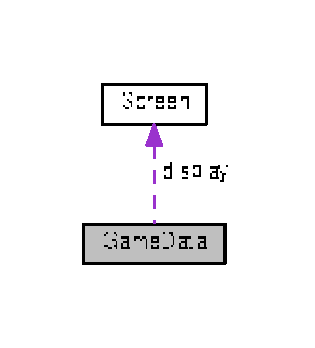
\includegraphics[width=151pt]{struct_game_data__coll__graph}
\end{center}
\end{figure}
\subsection*{Champs de données}
\begin{DoxyCompactItemize}
\item 
config\+\_\+t \textbf{ config\+File}
\item 
char $\ast$ \textbf{ app\+Name}
\item 
\textbf{ Game\+State} \textbf{ current\+\_\+state}
\item 
S\+D\+L\+\_\+\+Pixel\+Format $\ast$ \textbf{ pixelformat}
\item 
S\+D\+L\+\_\+\+Window $\ast$$\ast$ \textbf{ window}
\item 
int \textbf{ window\+\_\+width}
\item 
int \textbf{ window\+\_\+height}
\item 
unsigned int \textbf{ number\+Of\+Player}
\item 
S\+D\+L\+\_\+\+Renderer $\ast$$\ast$ \textbf{ renderer}
\item 
F\+P\+Smanager $\ast$$\ast$ \textbf{ manager}
\item 
\textbf{ Screen} \textbf{ display}
\end{DoxyCompactItemize}


\subsection{Description détaillée}
All data that the game must have to be ready 

Définition à la ligne 122 du fichier types.\+h.



\subsection{Documentation des champs}
\mbox{\label{struct_game_data_adefe7f7f4772ff051f1fdd5b6693d62c}} 
\index{Game\+Data@{Game\+Data}!app\+Name@{app\+Name}}
\index{app\+Name@{app\+Name}!Game\+Data@{Game\+Data}}
\subsubsection{app\+Name}
{\footnotesize\ttfamily char$\ast$ app\+Name}

{\bfseries Unused} {\bfseries nowadays}, will define the name of the window and app 

Définition à la ligne 125 du fichier types.\+h.

\mbox{\label{struct_game_data_af27d1b9ec87e6f2462c8b180de4de676}} 
\index{Game\+Data@{Game\+Data}!config\+File@{config\+File}}
\index{config\+File@{config\+File}!Game\+Data@{Game\+Data}}
\subsubsection{config\+File}
{\footnotesize\ttfamily config\+\_\+t config\+File}

{\bfseries Unused} {\bfseries nowadays}, but the data will be readable 

Définition à la ligne 124 du fichier types.\+h.

\mbox{\label{struct_game_data_a6ed9079283c2964b8f1c5bfccfc8727e}} 
\index{Game\+Data@{Game\+Data}!current\+\_\+state@{current\+\_\+state}}
\index{current\+\_\+state@{current\+\_\+state}!Game\+Data@{Game\+Data}}
\subsubsection{current\+\_\+state}
{\footnotesize\ttfamily \textbf{ Game\+State} current\+\_\+state}

Used for launch functions 

Définition à la ligne 126 du fichier types.\+h.

\mbox{\label{struct_game_data_ac64687171d64c7b90dac06fce8b37941}} 
\index{Game\+Data@{Game\+Data}!display@{display}}
\index{display@{display}!Game\+Data@{Game\+Data}}
\subsubsection{display}
{\footnotesize\ttfamily \textbf{ Screen} display}

\doxyref{Screen}{p.}{struct_screen} structure to displaying 

Définition à la ligne 134 du fichier types.\+h.

\mbox{\label{struct_game_data_abe833816151a2cf1782b845741049c02}} 
\index{Game\+Data@{Game\+Data}!manager@{manager}}
\index{manager@{manager}!Game\+Data@{Game\+Data}}
\subsubsection{manager}
{\footnotesize\ttfamily F\+P\+Smanager$\ast$$\ast$ manager}

Pointer to the F\+PS manager of the game 

Définition à la ligne 133 du fichier types.\+h.

\mbox{\label{struct_game_data_ac38c6c1d6a4e97b6882c0a32036802e1}} 
\index{Game\+Data@{Game\+Data}!number\+Of\+Player@{number\+Of\+Player}}
\index{number\+Of\+Player@{number\+Of\+Player}!Game\+Data@{Game\+Data}}
\subsubsection{number\+Of\+Player}
{\footnotesize\ttfamily unsigned int number\+Of\+Player}

Number of players that plays 

Définition à la ligne 131 du fichier types.\+h.

\mbox{\label{struct_game_data_a8a7fabd77cba73c77e75ae861ebe1c4d}} 
\index{Game\+Data@{Game\+Data}!pixelformat@{pixelformat}}
\index{pixelformat@{pixelformat}!Game\+Data@{Game\+Data}}
\subsubsection{pixelformat}
{\footnotesize\ttfamily S\+D\+L\+\_\+\+Pixel\+Format$\ast$ pixelformat}

Pixel format of the screen 

Définition à la ligne 127 du fichier types.\+h.

\mbox{\label{struct_game_data_aaa07ec38523f6fba243ce04fdd7f4619}} 
\index{Game\+Data@{Game\+Data}!renderer@{renderer}}
\index{renderer@{renderer}!Game\+Data@{Game\+Data}}
\subsubsection{renderer}
{\footnotesize\ttfamily S\+D\+L\+\_\+\+Renderer$\ast$$\ast$ renderer}

Pointer to the renderer 

Définition à la ligne 132 du fichier types.\+h.

\mbox{\label{struct_game_data_ad6bf7691ca1d4c87c4118cc76da2b264}} 
\index{Game\+Data@{Game\+Data}!window@{window}}
\index{window@{window}!Game\+Data@{Game\+Data}}
\subsubsection{window}
{\footnotesize\ttfamily S\+D\+L\+\_\+\+Window$\ast$$\ast$ window}

Pointer to the main window 

Définition à la ligne 128 du fichier types.\+h.

\mbox{\label{struct_game_data_aca33f926b061680d857699a22f676418}} 
\index{Game\+Data@{Game\+Data}!window\+\_\+height@{window\+\_\+height}}
\index{window\+\_\+height@{window\+\_\+height}!Game\+Data@{Game\+Data}}
\subsubsection{window\+\_\+height}
{\footnotesize\ttfamily int window\+\_\+height}

Window height in pixels 

Définition à la ligne 130 du fichier types.\+h.

\mbox{\label{struct_game_data_a0e2e740afd510cfe652a1836ffbad209}} 
\index{Game\+Data@{Game\+Data}!window\+\_\+width@{window\+\_\+width}}
\index{window\+\_\+width@{window\+\_\+width}!Game\+Data@{Game\+Data}}
\subsubsection{window\+\_\+width}
{\footnotesize\ttfamily int window\+\_\+width}

Window width in pixels 

Définition à la ligne 129 du fichier types.\+h.



La documentation de cette structure a été générée à partir du fichier suivant \+:\begin{DoxyCompactItemize}
\item 
\textbf{ types.\+h}\end{DoxyCompactItemize}

\section{Référence de la structure painter}
\label{structpainter}\index{painter@{painter}}


{\ttfamily \#include $<$types.\+h$>$}

\subsection*{Champs de données}
\begin{DoxyCompactItemize}
\item 
S\+D\+L\+\_\+\+Texture $\ast$ \textbf{ sprite\+Right}
\item 
S\+D\+L\+\_\+\+Texture $\ast$ \textbf{ sprite\+Left}
\item 
S\+D\+L\+\_\+\+Texture $\ast$$\ast$ \textbf{ active\+Sprit}
\item 
S\+D\+L\+\_\+\+Rect \textbf{ position}
\item 
S\+D\+L\+\_\+\+Keycode \textbf{ keys} [\textbf{ C\+T\+R\+L\+\_\+\+K\+E\+Y\+S\+\_\+\+N\+U\+M\+B\+ER}]
\item 
int \textbf{ brush\+Size}
\item 
Uint32 \textbf{ color}
\item 
S\+D\+L\+\_\+\+Color \textbf{ struct\+\_\+color}
\end{DoxyCompactItemize}


\subsection{Description détaillée}
Structure of a painter used everywhere. 

Définition à la ligne 142 du fichier types.\+h.



\subsection{Documentation des champs}
\mbox{\label{structpainter_a386313f47e956f1544cb6bcd2416836c}} 
\index{painter@{painter}!active\+Sprit@{active\+Sprit}}
\index{active\+Sprit@{active\+Sprit}!painter@{painter}}
\subsubsection{active\+Sprit}
{\footnotesize\ttfamily S\+D\+L\+\_\+\+Texture$\ast$$\ast$ active\+Sprit}

The sprite that is actually used 

Définition à la ligne 146 du fichier types.\+h.

\mbox{\label{structpainter_a9a97e37d5842d96acd10398a11107e96}} 
\index{painter@{painter}!brush\+Size@{brush\+Size}}
\index{brush\+Size@{brush\+Size}!painter@{painter}}
\subsubsection{brush\+Size}
{\footnotesize\ttfamily int brush\+Size}

Size of the brush of the painter 

Définition à la ligne 157 du fichier types.\+h.

\mbox{\label{structpainter_afd133e412238ed9f1e3ba52397115e8d}} 
\index{painter@{painter}!color@{color}}
\index{color@{color}!painter@{painter}}
\subsubsection{color}
{\footnotesize\ttfamily Uint32 color}

Coded R\+GB color of the painter 

Définition à la ligne 160 du fichier types.\+h.

\mbox{\label{structpainter_aaf7678c8bdea5f0a614d6bdb5af675fb}} 
\index{painter@{painter}!keys@{keys}}
\index{keys@{keys}!painter@{painter}}
\subsubsection{keys}
{\footnotesize\ttfamily S\+D\+L\+\_\+\+Keycode keys[\textbf{ C\+T\+R\+L\+\_\+\+K\+E\+Y\+S\+\_\+\+N\+U\+M\+B\+ER}]}

The control keys to move the painter 

Définition à la ligne 155 du fichier types.\+h.

\mbox{\label{structpainter_ac06cf6a292dc0e70e28b394fa481aef2}} 
\index{painter@{painter}!position@{position}}
\index{position@{position}!painter@{painter}}
\subsubsection{position}
{\footnotesize\ttfamily S\+D\+L\+\_\+\+Rect position}



The position and size of the player. 

Actually, the {\bfseries x} and {\bfseries y} members of the S\+D\+L\+\_\+\+Rect struct are used for position and the {\bfseries h} and {\bfseries w} members of the S\+D\+L\+\_\+\+Rect struct are equals to brush\+Size 

Définition à la ligne 154 du fichier types.\+h.

\mbox{\label{structpainter_a6172789122e545529f4a04419a0835f7}} 
\index{painter@{painter}!sprite\+Left@{sprite\+Left}}
\index{sprite\+Left@{sprite\+Left}!painter@{painter}}
\subsubsection{sprite\+Left}
{\footnotesize\ttfamily S\+D\+L\+\_\+\+Texture$\ast$ sprite\+Left}

The sprite when the painter is moving to the left 

Définition à la ligne 145 du fichier types.\+h.

\mbox{\label{structpainter_a9e331a61bff9303277f1d5666aa85c4d}} 
\index{painter@{painter}!sprite\+Right@{sprite\+Right}}
\index{sprite\+Right@{sprite\+Right}!painter@{painter}}
\subsubsection{sprite\+Right}
{\footnotesize\ttfamily S\+D\+L\+\_\+\+Texture$\ast$ sprite\+Right}

The sprite when the painter is moving to the right 

Définition à la ligne 144 du fichier types.\+h.

\mbox{\label{structpainter_ad40888d04f08a9b49fd8c442327fddef}} 
\index{painter@{painter}!struct\+\_\+color@{struct\+\_\+color}}
\index{struct\+\_\+color@{struct\+\_\+color}!painter@{painter}}
\subsubsection{struct\+\_\+color}
{\footnotesize\ttfamily S\+D\+L\+\_\+\+Color struct\+\_\+color}

Detailled R\+G\+BA color of the painter 

Définition à la ligne 161 du fichier types.\+h.



La documentation de cette structure a été générée à partir du fichier suivant \+:\begin{DoxyCompactItemize}
\item 
\textbf{ types.\+h}\end{DoxyCompactItemize}

\section{Référence de la structure Player}
\label{struct_player}\index{Player@{Player}}


{\ttfamily \#include $<$types.\+h$>$}



\subsection{Description détaillée}
Structure of a \doxyref{Player}{p.}{struct_player}. 

La documentation de cette structure a été générée à partir du fichier suivant \+:\begin{DoxyCompactItemize}
\item 
\textbf{ types.\+h}\end{DoxyCompactItemize}

\section{Référence de la structure player}
\label{structplayer}\index{player@{player}}


Graphe de collaboration de player\+:
\nopagebreak
\begin{figure}[H]
\begin{center}
\leavevmode
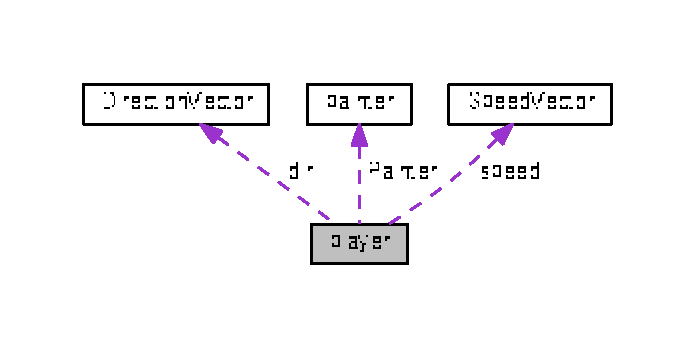
\includegraphics[width=334pt]{structplayer__coll__graph}
\end{center}
\end{figure}
\subsection*{Champs de données}
\begin{DoxyCompactItemize}
\item 
\textbf{ painter} $\ast$ \textbf{ Painter}
\item 
S\+D\+L\+\_\+bool \textbf{ isdef}
\item 
char \textbf{ name} [\textbf{ N\+A\+M\+E\+\_\+\+S\+T\+R\+I\+N\+G\+\_\+\+M\+AX}]
\item 
char \textbf{ id}
\item 
double \textbf{ scoreP}
\item 
\textbf{ Speed\+Vector} \textbf{ speed}
\item 
\textbf{ Direction\+Vector} \textbf{ dir}
\end{DoxyCompactItemize}


\subsection{Description détaillée}


Définition à la ligne 168 du fichier types.\+h.



\subsection{Documentation des champs}
\mbox{\label{structplayer_ac937d4dbbc71f2f0eb17958c8f6932bf}} 
\index{player@{player}!dir@{dir}}
\index{dir@{dir}!player@{player}}
\subsubsection{dir}
{\footnotesize\ttfamily \textbf{ Direction\+Vector} dir}

The direction of the player (8 possibility) \begin{DoxyRefDesc}{A faire}
\item[\textbf{ A faire}]Make the direction totally vectorial on a circle \end{DoxyRefDesc}


Définition à la ligne 180 du fichier types.\+h.

\mbox{\label{structplayer_af749ccd9c242573390416d80accd7b39}} 
\index{player@{player}!id@{id}}
\index{id@{id}!player@{player}}
\subsubsection{id}
{\footnotesize\ttfamily char id}

Identification number of the player (1 to M\+A\+X\+\_\+\+P\+L\+A\+Y\+E\+R\+S\+\_\+\+N\+U\+M\+B\+ER) 

Définition à la ligne 173 du fichier types.\+h.

\mbox{\label{structplayer_aae6bfe6d9f5f28bd749d1466831bb9cc}} 
\index{player@{player}!isdef@{isdef}}
\index{isdef@{isdef}!player@{player}}
\subsubsection{isdef}
{\footnotesize\ttfamily S\+D\+L\+\_\+bool isdef}

indicator of player existence 

Définition à la ligne 171 du fichier types.\+h.

\mbox{\label{structplayer_aea70c16e5e32ea53dfaf90630abe24ee}} 
\index{player@{player}!name@{name}}
\index{name@{name}!player@{player}}
\subsubsection{name}
{\footnotesize\ttfamily char name[\textbf{ N\+A\+M\+E\+\_\+\+S\+T\+R\+I\+N\+G\+\_\+\+M\+AX}]}

String of N\+A\+M\+E\+\_\+\+S\+T\+R\+I\+N\+G\+\_\+\+M\+AX chars to store the player name 

Définition à la ligne 172 du fichier types.\+h.

\mbox{\label{structplayer_aa718f83164f47e0716676b0aa8df07ec}} 
\index{player@{player}!Painter@{Painter}}
\index{Painter@{Painter}!player@{player}}
\subsubsection{Painter}
{\footnotesize\ttfamily \textbf{ painter}$\ast$ Painter}

pointer to the painter of the \doxyref{Player}{p.}{struct_player} 

Définition à la ligne 170 du fichier types.\+h.

\mbox{\label{structplayer_a260e160fd2a4cc082beb01802438dc13}} 
\index{player@{player}!scoreP@{scoreP}}
\index{scoreP@{scoreP}!player@{player}}
\subsubsection{scoreP}
{\footnotesize\ttfamily double scoreP}

Score of the player.

\begin{DoxyRefDesc}{A faire}
\item[\textbf{ A faire}]Why double ? Long int isn\textquotesingle{}t sufficient ? \end{DoxyRefDesc}


Définition à la ligne 174 du fichier types.\+h.

\mbox{\label{structplayer_a5b7b86d6d2233aa5cb90962f602a20a1}} 
\index{player@{player}!speed@{speed}}
\index{speed@{speed}!player@{player}}
\subsubsection{speed}
{\footnotesize\ttfamily \textbf{ Speed\+Vector} speed}

The speed of the player 

Définition à la ligne 179 du fichier types.\+h.



La documentation de cette structure a été générée à partir du fichier suivant \+:\begin{DoxyCompactItemize}
\item 
\textbf{ types.\+h}\end{DoxyCompactItemize}

\section{Référence de la structure Screen}
\label{struct_screen}\index{Screen@{Screen}}


{\ttfamily \#include $<$types.\+h$>$}

\subsection*{Champs de données}
\begin{DoxyCompactItemize}
\item 
S\+D\+L\+\_\+\+Texture $\ast$ \textbf{ background}
\item 
S\+D\+L\+\_\+\+Texture $\ast$ \textbf{ foreground}
\item 
S\+D\+L\+\_\+\+Surface $\ast$ \textbf{ readable\+\_\+foreground}
\end{DoxyCompactItemize}


\subsection{Description détaillée}
Define the screen of the game \begin{DoxyRefDesc}{A faire}
\item[\textbf{ A faire}]Add the G\+UI zone \end{DoxyRefDesc}


Définition à la ligne 105 du fichier types.\+h.



\subsection{Documentation des champs}
\mbox{\label{struct_screen_aa6506cd10a348128d0d73bb4dfa58dd5}} 
\index{Screen@{Screen}!background@{background}}
\index{background@{background}!Screen@{Screen}}
\subsubsection{background}
{\footnotesize\ttfamily S\+D\+L\+\_\+\+Texture$\ast$ background}

Background, a picture or a sample color 

Définition à la ligne 107 du fichier types.\+h.

\mbox{\label{struct_screen_acc7002f76faedbe16b828b373a96ee5b}} 
\index{Screen@{Screen}!foreground@{foreground}}
\index{foreground@{foreground}!Screen@{Screen}}
\subsubsection{foreground}
{\footnotesize\ttfamily S\+D\+L\+\_\+\+Texture$\ast$ foreground}

Layer where paint lines will be displayed 

Définition à la ligne 108 du fichier types.\+h.

\mbox{\label{struct_screen_ada24f13ca94adc152b2a1a58473405c0}} 
\index{Screen@{Screen}!readable\+\_\+foreground@{readable\+\_\+foreground}}
\index{readable\+\_\+foreground@{readable\+\_\+foreground}!Screen@{Screen}}
\subsubsection{readable\+\_\+foreground}
{\footnotesize\ttfamily S\+D\+L\+\_\+\+Surface$\ast$ readable\+\_\+foreground}

Surface used for pixel manipulating 

Définition à la ligne 109 du fichier types.\+h.



La documentation de cette structure a été générée à partir du fichier suivant \+:\begin{DoxyCompactItemize}
\item 
\textbf{ types.\+h}\end{DoxyCompactItemize}

\section{Référence de la structure Speed\+Vector}
\label{struct_speed_vector}\index{Speed\+Vector@{Speed\+Vector}}


{\ttfamily \#include $<$types.\+h$>$}

\subsection*{Champs de données}
\begin{DoxyCompactItemize}
\item 
\textbf{ Speed} \textbf{ x}
\item 
\textbf{ Speed} \textbf{ y}
\end{DoxyCompactItemize}


\subsection{Description détaillée}
Speeds of a player, related to malus and bonus 

Définition à la ligne 94 du fichier types.\+h.



\subsection{Documentation des champs}
\mbox{\label{struct_speed_vector_a6eb82865dfa8817d407ad66fd781a231}} 
\index{Speed\+Vector@{Speed\+Vector}!x@{x}}
\index{x@{x}!Speed\+Vector@{Speed\+Vector}}
\subsubsection{x}
{\footnotesize\ttfamily \textbf{ Speed} x}

Speed on X-\/axis 

Définition à la ligne 96 du fichier types.\+h.

\mbox{\label{struct_speed_vector_a4850d889ee6534fb9a0974232d123827}} 
\index{Speed\+Vector@{Speed\+Vector}!y@{y}}
\index{y@{y}!Speed\+Vector@{Speed\+Vector}}
\subsubsection{y}
{\footnotesize\ttfamily \textbf{ Speed} y}

Speed on Y-\/axis 

Définition à la ligne 97 du fichier types.\+h.



La documentation de cette structure a été générée à partir du fichier suivant \+:\begin{DoxyCompactItemize}
\item 
\textbf{ types.\+h}\end{DoxyCompactItemize}

\chapter{Documentation des fichiers}
\section{Référence du fichier defines.\+h}
\label{defines_8h}\index{defines.\+h@{defines.\+h}}
Ce graphe montre quels fichiers incluent directement ou indirectement ce fichier \+:
\nopagebreak
\begin{figure}[H]
\begin{center}
\leavevmode
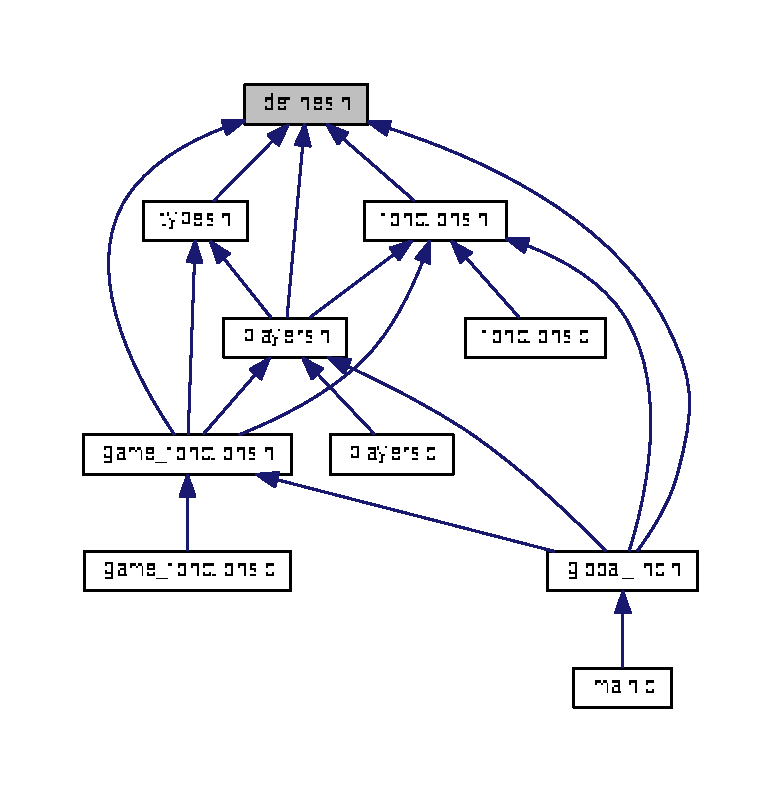
\includegraphics[width=350pt]{defines_8h__dep__incl}
\end{center}
\end{figure}
\subsection*{Macros}
\begin{DoxyCompactItemize}
\item 
\#define \textbf{ S\+C\+R\+E\+E\+N\+\_\+\+H\+E\+I\+G\+HT}~(1024)
\item 
\#define \textbf{ S\+C\+R\+E\+E\+N\+\_\+\+W\+I\+D\+TH}~(1080)
\item 
\#define \textbf{ S\+T\+R\+I\+N\+G\+\_\+\+S\+I\+ZE}~(40)
\item 
\#define \textbf{ K}~$\ast$(1000)
\item 
\#define \textbf{ C\+T\+R\+L\+\_\+\+K\+E\+Y\+S\+\_\+\+N\+U\+M\+B\+ER}~4
\item 
\#define \textbf{ M\+A\+X\+\_\+\+P\+L\+A\+Y\+E\+RS}~(4)
\item 
\#define \textbf{ N\+A\+M\+E\+\_\+\+S\+T\+R\+I\+N\+G\+\_\+\+M\+AX}~(32)
\item 
\#define \textbf{ T\+O\+\_\+\+U\+N\+D\+U\+M\+MY}~(1)
\item 
\#define \textbf{ N\+B\+\_\+\+I\+M\+G\+\_\+\+P\+E\+R\+\_\+\+S\+E\+C\+O\+ND}~(30)
\item 
\#define \textbf{ C\+L\+E\+A\+R\+\_\+\+B\+U\+F\+F\+ER}~do \{while(getchar() != \textquotesingle{}\textbackslash{}n\textquotesingle{});\}while(0)
\end{DoxyCompactItemize}


\subsection{Description détaillée}
Define all symbolic constants and some macros. 

\begin{DoxyAuthor}{Auteur}
Marius Monnier 
\end{DoxyAuthor}
\begin{DoxyVersion}{Version}
0.\+1 
\end{DoxyVersion}


\subsection{Documentation des macros}
\mbox{\label{defines_8h_aa28dd17f6f34a0944a90f741b0251239}} 
\index{defines.\+h@{defines.\+h}!C\+L\+E\+A\+R\+\_\+\+B\+U\+F\+F\+ER@{C\+L\+E\+A\+R\+\_\+\+B\+U\+F\+F\+ER}}
\index{C\+L\+E\+A\+R\+\_\+\+B\+U\+F\+F\+ER@{C\+L\+E\+A\+R\+\_\+\+B\+U\+F\+F\+ER}!defines.\+h@{defines.\+h}}
\subsubsection{C\+L\+E\+A\+R\+\_\+\+B\+U\+F\+F\+ER}
{\footnotesize\ttfamily \#define C\+L\+E\+A\+R\+\_\+\+B\+U\+F\+F\+ER~do \{while(getchar() != \textquotesingle{}\textbackslash{}n\textquotesingle{});\}while(0)}

Little protected macro to clear the buffer after or before a scanf for example 

Définition à la ligne 28 du fichier defines.\+h.

\mbox{\label{defines_8h_aad5c97fa552c0b5e940254a27cb04c94}} 
\index{defines.\+h@{defines.\+h}!C\+T\+R\+L\+\_\+\+K\+E\+Y\+S\+\_\+\+N\+U\+M\+B\+ER@{C\+T\+R\+L\+\_\+\+K\+E\+Y\+S\+\_\+\+N\+U\+M\+B\+ER}}
\index{C\+T\+R\+L\+\_\+\+K\+E\+Y\+S\+\_\+\+N\+U\+M\+B\+ER@{C\+T\+R\+L\+\_\+\+K\+E\+Y\+S\+\_\+\+N\+U\+M\+B\+ER}!defines.\+h@{defines.\+h}}
\subsubsection{C\+T\+R\+L\+\_\+\+K\+E\+Y\+S\+\_\+\+N\+U\+M\+B\+ER}
{\footnotesize\ttfamily \#define C\+T\+R\+L\+\_\+\+K\+E\+Y\+S\+\_\+\+N\+U\+M\+B\+ER~4}

Define number of control keys for a player 

Définition à la ligne 16 du fichier defines.\+h.

\mbox{\label{defines_8h_a97d832ae23af4f215e801e37e4f94254}} 
\index{defines.\+h@{defines.\+h}!K@{K}}
\index{K@{K}!defines.\+h@{defines.\+h}}
\subsubsection{K}
{\footnotesize\ttfamily \#define K~$\ast$(1000)}

Define a semi \char`\"{}converting\char`\"{} operator 

Définition à la ligne 15 du fichier defines.\+h.

\mbox{\label{defines_8h_a1c346c944e8204fd06dc057393c7c96d}} 
\index{defines.\+h@{defines.\+h}!M\+A\+X\+\_\+\+P\+L\+A\+Y\+E\+RS@{M\+A\+X\+\_\+\+P\+L\+A\+Y\+E\+RS}}
\index{M\+A\+X\+\_\+\+P\+L\+A\+Y\+E\+RS@{M\+A\+X\+\_\+\+P\+L\+A\+Y\+E\+RS}!defines.\+h@{defines.\+h}}
\subsubsection{M\+A\+X\+\_\+\+P\+L\+A\+Y\+E\+RS}
{\footnotesize\ttfamily \#define M\+A\+X\+\_\+\+P\+L\+A\+Y\+E\+RS~(4)}

Define maximum number of players 

Définition à la ligne 18 du fichier defines.\+h.

\mbox{\label{defines_8h_a049c2ad0e3ddad098c8c4bc484ff49dc}} 
\index{defines.\+h@{defines.\+h}!N\+A\+M\+E\+\_\+\+S\+T\+R\+I\+N\+G\+\_\+\+M\+AX@{N\+A\+M\+E\+\_\+\+S\+T\+R\+I\+N\+G\+\_\+\+M\+AX}}
\index{N\+A\+M\+E\+\_\+\+S\+T\+R\+I\+N\+G\+\_\+\+M\+AX@{N\+A\+M\+E\+\_\+\+S\+T\+R\+I\+N\+G\+\_\+\+M\+AX}!defines.\+h@{defines.\+h}}
\subsubsection{N\+A\+M\+E\+\_\+\+S\+T\+R\+I\+N\+G\+\_\+\+M\+AX}
{\footnotesize\ttfamily \#define N\+A\+M\+E\+\_\+\+S\+T\+R\+I\+N\+G\+\_\+\+M\+AX~(32)}

Define maximum size of player\textquotesingle{}s name 

Définition à la ligne 19 du fichier defines.\+h.

\mbox{\label{defines_8h_ad10cb0832fe62a5b27a6a9a3571cc6ca}} 
\index{defines.\+h@{defines.\+h}!N\+B\+\_\+\+I\+M\+G\+\_\+\+P\+E\+R\+\_\+\+S\+E\+C\+O\+ND@{N\+B\+\_\+\+I\+M\+G\+\_\+\+P\+E\+R\+\_\+\+S\+E\+C\+O\+ND}}
\index{N\+B\+\_\+\+I\+M\+G\+\_\+\+P\+E\+R\+\_\+\+S\+E\+C\+O\+ND@{N\+B\+\_\+\+I\+M\+G\+\_\+\+P\+E\+R\+\_\+\+S\+E\+C\+O\+ND}!defines.\+h@{defines.\+h}}
\subsubsection{N\+B\+\_\+\+I\+M\+G\+\_\+\+P\+E\+R\+\_\+\+S\+E\+C\+O\+ND}
{\footnotesize\ttfamily \#define N\+B\+\_\+\+I\+M\+G\+\_\+\+P\+E\+R\+\_\+\+S\+E\+C\+O\+ND~(30)}

Number of img per second, for the fps manager 

Définition à la ligne 22 du fichier defines.\+h.

\mbox{\label{defines_8h_a6974d08a74da681b3957b2fead2608b8}} 
\index{defines.\+h@{defines.\+h}!S\+C\+R\+E\+E\+N\+\_\+\+H\+E\+I\+G\+HT@{S\+C\+R\+E\+E\+N\+\_\+\+H\+E\+I\+G\+HT}}
\index{S\+C\+R\+E\+E\+N\+\_\+\+H\+E\+I\+G\+HT@{S\+C\+R\+E\+E\+N\+\_\+\+H\+E\+I\+G\+HT}!defines.\+h@{defines.\+h}}
\subsubsection{S\+C\+R\+E\+E\+N\+\_\+\+H\+E\+I\+G\+HT}
{\footnotesize\ttfamily \#define S\+C\+R\+E\+E\+N\+\_\+\+H\+E\+I\+G\+HT~(1024)}

Define window height 

Définition à la ligne 10 du fichier defines.\+h.

\mbox{\label{defines_8h_a2cd109632a6dcccaa80b43561b1ab700}} 
\index{defines.\+h@{defines.\+h}!S\+C\+R\+E\+E\+N\+\_\+\+W\+I\+D\+TH@{S\+C\+R\+E\+E\+N\+\_\+\+W\+I\+D\+TH}}
\index{S\+C\+R\+E\+E\+N\+\_\+\+W\+I\+D\+TH@{S\+C\+R\+E\+E\+N\+\_\+\+W\+I\+D\+TH}!defines.\+h@{defines.\+h}}
\subsubsection{S\+C\+R\+E\+E\+N\+\_\+\+W\+I\+D\+TH}
{\footnotesize\ttfamily \#define S\+C\+R\+E\+E\+N\+\_\+\+W\+I\+D\+TH~(1080)}

Define window width 

Définition à la ligne 11 du fichier defines.\+h.

\mbox{\label{defines_8h_ad78224efe1d3fb39b67ca74ad9d9eec7}} 
\index{defines.\+h@{defines.\+h}!S\+T\+R\+I\+N\+G\+\_\+\+S\+I\+ZE@{S\+T\+R\+I\+N\+G\+\_\+\+S\+I\+ZE}}
\index{S\+T\+R\+I\+N\+G\+\_\+\+S\+I\+ZE@{S\+T\+R\+I\+N\+G\+\_\+\+S\+I\+ZE}!defines.\+h@{defines.\+h}}
\subsubsection{S\+T\+R\+I\+N\+G\+\_\+\+S\+I\+ZE}
{\footnotesize\ttfamily \#define S\+T\+R\+I\+N\+G\+\_\+\+S\+I\+ZE~(40)}

Define maximum size of strings in program 

Définition à la ligne 13 du fichier defines.\+h.

\mbox{\label{defines_8h_a7d95136fd756fcc08e4b94f27aa6e749}} 
\index{defines.\+h@{defines.\+h}!T\+O\+\_\+\+U\+N\+D\+U\+M\+MY@{T\+O\+\_\+\+U\+N\+D\+U\+M\+MY}}
\index{T\+O\+\_\+\+U\+N\+D\+U\+M\+MY@{T\+O\+\_\+\+U\+N\+D\+U\+M\+MY}!defines.\+h@{defines.\+h}}
\subsubsection{T\+O\+\_\+\+U\+N\+D\+U\+M\+MY}
{\footnotesize\ttfamily \#define T\+O\+\_\+\+U\+N\+D\+U\+M\+MY~(1)}

Operator for T\+O\+DO 

Définition à la ligne 20 du fichier defines.\+h.


\section{Référence du fichier fonctions.\+c}
\label{fonctions_8c}\index{fonctions.\+c@{fonctions.\+c}}
{\ttfamily \#include \char`\"{}fonctions.\+h\char`\"{}}\newline
Graphe des dépendances par inclusion de fonctions.\+c\+:
\nopagebreak
\begin{figure}[H]
\begin{center}
\leavevmode
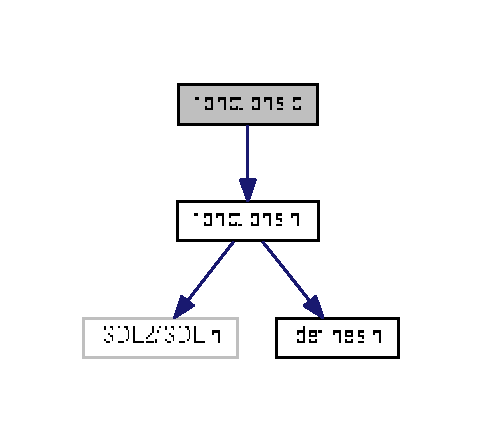
\includegraphics[width=232pt]{fonctions_8c__incl}
\end{center}
\end{figure}
\subsection*{Fonctions}
\begin{DoxyCompactItemize}
\item 
void \textbf{ str\+\_\+replace} (char $\ast$$\ast$s, int token, int replacement)
\item 
\mbox{\label{fonctions_8c_a100d09f9a57d44745299c28c63c98745}} 
void {\bfseries dummy} ()
\item 
int \textbf{ readline} (char $\ast$s, int n)
\item 
\mbox{\label{fonctions_8c_a48c6792c544a90cd7a552667ce5bba4a}} 
Uint32 {\bfseries get\+Pixel} (S\+D\+L\+\_\+\+Surface $\ast$surface, int x, int y)
\item 
void \textbf{ clear\+\_\+texture} (S\+D\+L\+\_\+\+Texture $\ast$texture, S\+D\+L\+\_\+\+Renderer $\ast$renderer)
\item 
int \textbf{ set\+Render\+Draw\+Color} (S\+D\+L\+\_\+\+Renderer $\ast$renderer, S\+D\+L\+\_\+\+Color $\ast$color)
\end{DoxyCompactItemize}


\subsection{Description détaillée}
Implementation of some functions that can be used anywhere. 

\begin{DoxyAuthor}{Auteur}
Marius Monnier 
\end{DoxyAuthor}
\begin{DoxyVersion}{Version}
0.\+1 
\end{DoxyVersion}


\subsection{Documentation des fonctions}
\mbox{\label{fonctions_8c_ab0852adabab2829b722da4fc549ac6a9}} 
\index{fonctions.\+c@{fonctions.\+c}!clear\+\_\+texture@{clear\+\_\+texture}}
\index{clear\+\_\+texture@{clear\+\_\+texture}!fonctions.\+c@{fonctions.\+c}}
\subsubsection{clear\+\_\+texture()}
{\footnotesize\ttfamily void clear\+\_\+texture (\begin{DoxyParamCaption}\item[{S\+D\+L\+\_\+\+Texture $\ast$}]{texture,  }\item[{S\+D\+L\+\_\+\+Renderer $\ast$}]{renderer }\end{DoxyParamCaption})}



Function that set a texture to black transparent texture (clear everything) 


\begin{DoxyParams}{Paramètres}
{\em texture} & pointer to the texture \\
\hline
{\em renderer} & pointer to the renderer that is used \\
\hline
\end{DoxyParams}


Définition à la ligne 104 du fichier fonctions.\+c.

\mbox{\label{fonctions_8c_afe286242e48f523265fd5fcdae3f7358}} 
\index{fonctions.\+c@{fonctions.\+c}!readline@{readline}}
\index{readline@{readline}!fonctions.\+c@{fonctions.\+c}}
\subsubsection{readline()}
{\footnotesize\ttfamily int readline (\begin{DoxyParamCaption}\item[{char $\ast$}]{s,  }\item[{int}]{n }\end{DoxyParamCaption})}



Function that read a line securely and make it a valid string. 


\begin{DoxyParams}{Paramètres}
{\em s} & pointer that will store the string \\
\hline
{\em n} & number of character that will be read \\
\hline
\end{DoxyParams}
\begin{DoxyReturn}{Renvoie}
E\+X\+I\+T\+\_\+\+S\+U\+C\+C\+E\+SS if success, E\+X\+I\+T\+\_\+\+F\+A\+I\+L\+U\+RE otherwise.
\end{DoxyReturn}
That function use fgets to create the string, and replace the final \textquotesingle{}~\newline
\textquotesingle{} with a \textquotesingle{}\textbackslash{}0\textquotesingle{} to make the string valid. \begin{DoxyRefDesc}{A faire}
\item[\textbf{ A faire}]A way to describe the error ? \end{DoxyRefDesc}


Définition à la ligne 44 du fichier fonctions.\+c.

Voici le graphe d\textquotesingle{}appel pour cette fonction \+:
\nopagebreak
\begin{figure}[H]
\begin{center}
\leavevmode
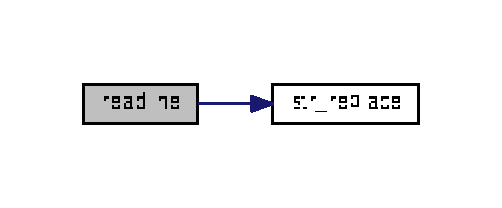
\includegraphics[width=241pt]{fonctions_8c_afe286242e48f523265fd5fcdae3f7358_cgraph}
\end{center}
\end{figure}
\mbox{\label{fonctions_8c_ad8ec5206bc6a89f1b70d8895523b7919}} 
\index{fonctions.\+c@{fonctions.\+c}!set\+Render\+Draw\+Color@{set\+Render\+Draw\+Color}}
\index{set\+Render\+Draw\+Color@{set\+Render\+Draw\+Color}!fonctions.\+c@{fonctions.\+c}}
\subsubsection{set\+Render\+Draw\+Color()}
{\footnotesize\ttfamily int set\+Render\+Draw\+Color (\begin{DoxyParamCaption}\item[{S\+D\+L\+\_\+\+Renderer $\ast$}]{renderer,  }\item[{S\+D\+L\+\_\+\+Color $\ast$}]{color }\end{DoxyParamCaption})}



Convenience function to set the color from a struct. 


\begin{DoxyParams}{Paramètres}
{\em renderer} & pointer to the renderer that will be modified \\
\hline
{\em color} & Structure that store the color components \\
\hline
\end{DoxyParams}


Définition à la ligne 119 du fichier fonctions.\+c.

\mbox{\label{fonctions_8c_afd361e8fd7c973935407a430d0c609a5}} 
\index{fonctions.\+c@{fonctions.\+c}!str\+\_\+replace@{str\+\_\+replace}}
\index{str\+\_\+replace@{str\+\_\+replace}!fonctions.\+c@{fonctions.\+c}}
\subsubsection{str\+\_\+replace()}
{\footnotesize\ttfamily void str\+\_\+replace (\begin{DoxyParamCaption}\item[{char $\ast$$\ast$}]{s,  }\item[{int}]{token,  }\item[{int}]{replacement }\end{DoxyParamCaption})}



Function that replace one token by another in a given string. 


\begin{DoxyParams}{Paramètres}
{\em s} & pointer to the string that will be modified \\
\hline
{\em token} & Character to search in string \\
\hline
{\em replacement} & Character that will replace token\\
\hline
\end{DoxyParams}
That function did not return something because the original string is modified. We use strchr() to find the token.

\begin{DoxyRefDesc}{A faire}
\item[\textbf{ A faire}]Some validity tests for token and replacement. \end{DoxyRefDesc}


Définition à la ligne 19 du fichier fonctions.\+c.

Voici le graphe des appelants de cette fonction \+:
\nopagebreak
\begin{figure}[H]
\begin{center}
\leavevmode
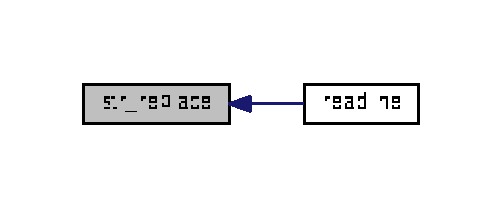
\includegraphics[width=241pt]{fonctions_8c_afd361e8fd7c973935407a430d0c609a5_icgraph}
\end{center}
\end{figure}

\section{Référence du fichier fonctions.\+h}
\label{fonctions_8h}\index{fonctions.\+h@{fonctions.\+h}}
{\ttfamily \#include $<$S\+D\+L2/\+S\+D\+L.\+h$>$}\newline
{\ttfamily \#include \char`\"{}defines.\+h\char`\"{}}\newline
Graphe des dépendances par inclusion de fonctions.\+h\+:
\nopagebreak
\begin{figure}[H]
\begin{center}
\leavevmode
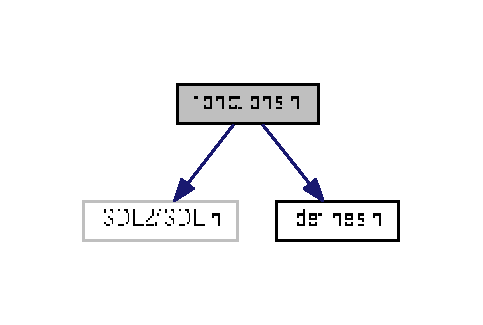
\includegraphics[width=232pt]{fonctions_8h__incl}
\end{center}
\end{figure}
Ce graphe montre quels fichiers incluent directement ou indirectement ce fichier \+:
\nopagebreak
\begin{figure}[H]
\begin{center}
\leavevmode
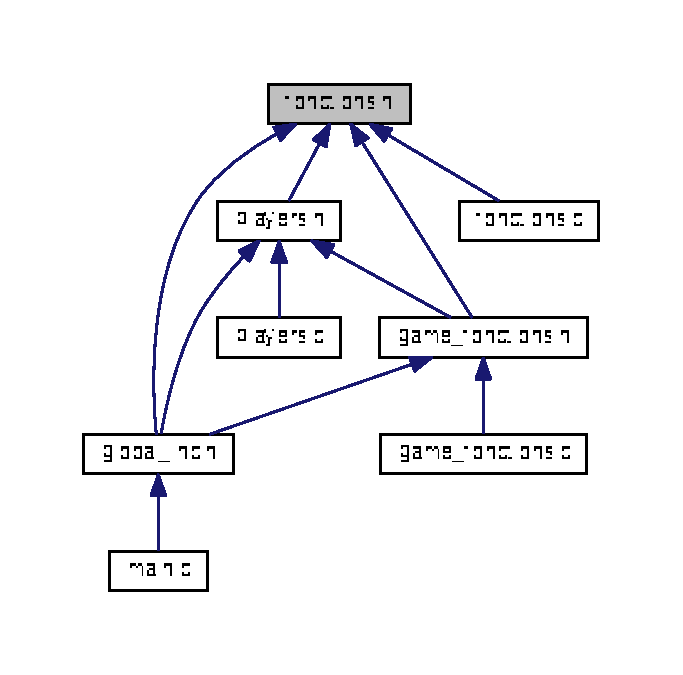
\includegraphics[width=328pt]{fonctions_8h__dep__incl}
\end{center}
\end{figure}
\subsection*{Fonctions}
\begin{DoxyCompactItemize}
\item 
\mbox{\label{fonctions_8h_a48c6792c544a90cd7a552667ce5bba4a}} 
Uint32 {\bfseries get\+Pixel} (S\+D\+L\+\_\+\+Surface $\ast$surface, int x, int y)
\item 
void \textbf{ str\+\_\+replace} (char $\ast$$\ast$s, int token, int replacement)
\item 
int \textbf{ readline} (char $\ast$s, int n)
\item 
\mbox{\label{fonctions_8h_a100d09f9a57d44745299c28c63c98745}} 
void {\bfseries dummy} ()
\item 
void \textbf{ clear\+\_\+texture} (S\+D\+L\+\_\+\+Texture $\ast$texture, S\+D\+L\+\_\+\+Renderer $\ast$renderer)
\item 
int \textbf{ set\+Render\+Draw\+Color} (S\+D\+L\+\_\+\+Renderer $\ast$renderer, S\+D\+L\+\_\+\+Color $\ast$color)
\end{DoxyCompactItemize}


\subsection{Description détaillée}
Define prototypes of common functions and includes other Headers files. 

\begin{DoxyAuthor}{Auteur}
Marius Monnier 
\end{DoxyAuthor}
\begin{DoxyVersion}{Version}
0.\+1 
\end{DoxyVersion}


\subsection{Documentation des fonctions}
\mbox{\label{fonctions_8h_ab0852adabab2829b722da4fc549ac6a9}} 
\index{fonctions.\+h@{fonctions.\+h}!clear\+\_\+texture@{clear\+\_\+texture}}
\index{clear\+\_\+texture@{clear\+\_\+texture}!fonctions.\+h@{fonctions.\+h}}
\subsubsection{clear\+\_\+texture()}
{\footnotesize\ttfamily void clear\+\_\+texture (\begin{DoxyParamCaption}\item[{S\+D\+L\+\_\+\+Texture $\ast$}]{texture,  }\item[{S\+D\+L\+\_\+\+Renderer $\ast$}]{renderer }\end{DoxyParamCaption})}



Function that set a texture to black transparent texture (clear everything) 


\begin{DoxyParams}{Paramètres}
{\em texture} & pointer to the texture \\
\hline
{\em renderer} & pointer to the renderer that is used \\
\hline
\end{DoxyParams}


Définition à la ligne 104 du fichier fonctions.\+c.

\mbox{\label{fonctions_8h_afe286242e48f523265fd5fcdae3f7358}} 
\index{fonctions.\+h@{fonctions.\+h}!readline@{readline}}
\index{readline@{readline}!fonctions.\+h@{fonctions.\+h}}
\subsubsection{readline()}
{\footnotesize\ttfamily int readline (\begin{DoxyParamCaption}\item[{char $\ast$}]{s,  }\item[{int}]{n }\end{DoxyParamCaption})}



Function that read a line securely and make it a valid string. 


\begin{DoxyParams}{Paramètres}
{\em s} & pointer that will store the string \\
\hline
{\em n} & number of character that will be read \\
\hline
\end{DoxyParams}
\begin{DoxyReturn}{Renvoie}
E\+X\+I\+T\+\_\+\+S\+U\+C\+C\+E\+SS if success, E\+X\+I\+T\+\_\+\+F\+A\+I\+L\+U\+RE otherwise.
\end{DoxyReturn}
That function use fgets to create the string, and replace the final \textquotesingle{}~\newline
\textquotesingle{} with a \textquotesingle{}\textbackslash{}0\textquotesingle{} to make the string valid. \begin{DoxyRefDesc}{A faire}
\item[\textbf{ A faire}]A way to describe the error ? \end{DoxyRefDesc}


Définition à la ligne 44 du fichier fonctions.\+c.

Voici le graphe d\textquotesingle{}appel pour cette fonction \+:
\nopagebreak
\begin{figure}[H]
\begin{center}
\leavevmode
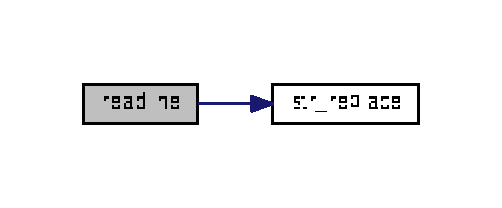
\includegraphics[width=241pt]{fonctions_8h_afe286242e48f523265fd5fcdae3f7358_cgraph}
\end{center}
\end{figure}
\mbox{\label{fonctions_8h_ad8ec5206bc6a89f1b70d8895523b7919}} 
\index{fonctions.\+h@{fonctions.\+h}!set\+Render\+Draw\+Color@{set\+Render\+Draw\+Color}}
\index{set\+Render\+Draw\+Color@{set\+Render\+Draw\+Color}!fonctions.\+h@{fonctions.\+h}}
\subsubsection{set\+Render\+Draw\+Color()}
{\footnotesize\ttfamily int set\+Render\+Draw\+Color (\begin{DoxyParamCaption}\item[{S\+D\+L\+\_\+\+Renderer $\ast$}]{renderer,  }\item[{S\+D\+L\+\_\+\+Color $\ast$}]{color }\end{DoxyParamCaption})}



Convenience function to set the color from a struct. 


\begin{DoxyParams}{Paramètres}
{\em renderer} & pointer to the renderer that will be modified \\
\hline
{\em color} & Structure that store the color components \\
\hline
\end{DoxyParams}


Définition à la ligne 119 du fichier fonctions.\+c.

\mbox{\label{fonctions_8h_afd361e8fd7c973935407a430d0c609a5}} 
\index{fonctions.\+h@{fonctions.\+h}!str\+\_\+replace@{str\+\_\+replace}}
\index{str\+\_\+replace@{str\+\_\+replace}!fonctions.\+h@{fonctions.\+h}}
\subsubsection{str\+\_\+replace()}
{\footnotesize\ttfamily void str\+\_\+replace (\begin{DoxyParamCaption}\item[{char $\ast$$\ast$}]{s,  }\item[{int}]{token,  }\item[{int}]{replacement }\end{DoxyParamCaption})}



Function that replace one token by another in a given string. 


\begin{DoxyParams}{Paramètres}
{\em s} & pointer to the string that will be modified \\
\hline
{\em token} & Character to search in string \\
\hline
{\em replacement} & Character that will replace token\\
\hline
\end{DoxyParams}
That function did not return something because the original string is modified. We use strchr() to find the token.

\begin{DoxyRefDesc}{A faire}
\item[\textbf{ A faire}]Some validity tests for token and replacement. \end{DoxyRefDesc}


Définition à la ligne 19 du fichier fonctions.\+c.

Voici le graphe des appelants de cette fonction \+:
\nopagebreak
\begin{figure}[H]
\begin{center}
\leavevmode
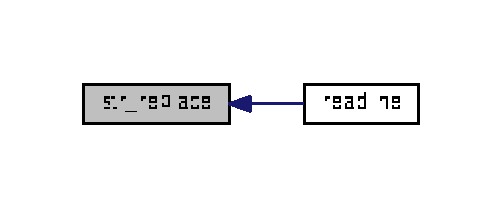
\includegraphics[width=241pt]{fonctions_8h_afd361e8fd7c973935407a430d0c609a5_icgraph}
\end{center}
\end{figure}

\section{Référence du fichier game\+\_\+fonctions.\+c}
\label{game__fonctions_8c}\index{game\+\_\+fonctions.\+c@{game\+\_\+fonctions.\+c}}
{\ttfamily \#include \char`\"{}game\+\_\+fonctions.\+h\char`\"{}}\newline
Graphe des dépendances par inclusion de game\+\_\+fonctions.\+c\+:
\nopagebreak
\begin{figure}[H]
\begin{center}
\leavevmode
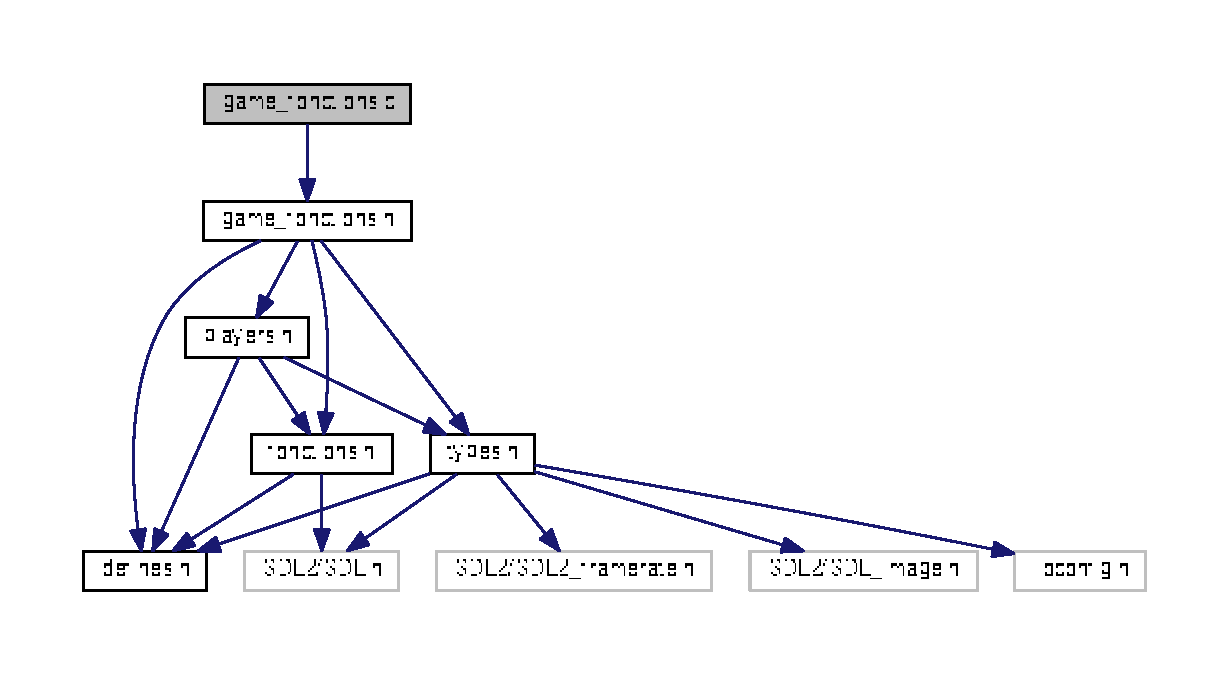
\includegraphics[width=350pt]{game__fonctions_8c__incl}
\end{center}
\end{figure}
\subsection*{Fonctions}
\begin{DoxyCompactItemize}
\item 
\mbox{\label{game__fonctions_8c_ab3538182e6fae78c414c6b371c6f9b77}} 
void {\bfseries launch\+\_\+menu} (void)
\item 
\mbox{\label{game__fonctions_8c_ae1e52800cf2d4cb84e2c71d6af390622}} 
void {\bfseries launch\+\_\+game} (void)
\item 
\mbox{\label{game__fonctions_8c_af44b6382ab2dcccef07d61d735915bfa}} 
void {\bfseries launch\+\_\+replay} (void)
\item 
\mbox{\label{game__fonctions_8c_a5c9adc58626460dbf4f5280f43cafebf}} 
\textbf{ Game\+Data} $\ast$ {\bfseries create\+Game\+Data} (S\+D\+L\+\_\+\+Window $\ast$$\ast$window, S\+D\+L\+\_\+\+Renderer $\ast$$\ast$renderer, char $\ast$app\+Name)
\item 
\mbox{\label{game__fonctions_8c_a4dd7e919802a1f82dd6020412e5db80f}} 
int {\bfseries init\+S\+D\+L\+Systems} (F\+P\+Smanager $\ast$manager)
\item 
\mbox{\label{game__fonctions_8c_ae38078a115bc28d56f1e559a188e7437}} 
int {\bfseries init\+Window\+And\+Renderer} (S\+D\+L\+\_\+\+Window $\ast$$\ast$window, S\+D\+L\+\_\+\+Renderer $\ast$$\ast$renderer, const unsigned int width, const unsigned int height, const char $\ast$title)
\end{DoxyCompactItemize}
\subsection*{Variables}
\begin{DoxyCompactItemize}
\item 
\textbf{ Game\+Data} $\ast$ \textbf{ data}
\item 
\mbox{\label{game__fonctions_8c_aa6e0d10ac9dacf902c351a3cbb8a474d}} 
\textbf{ player} $\ast$ {\bfseries players} [$\,$]
\end{DoxyCompactItemize}


\subsection{Description détaillée}
Implement static and public core parts. 

\begin{DoxyAuthor}{Auteur}
Marius Monnier 
\end{DoxyAuthor}
\begin{DoxyVersion}{Version}
0.\+1 
\end{DoxyVersion}


\subsection{Documentation des variables}
\mbox{\label{game__fonctions_8c_a882ad77a7df764b098f98136eb56a83a}} 
\index{game\+\_\+fonctions.\+c@{game\+\_\+fonctions.\+c}!data@{data}}
\index{data@{data}!game\+\_\+fonctions.\+c@{game\+\_\+fonctions.\+c}}
\subsubsection{data}
{\footnotesize\ttfamily \textbf{ Game\+Data}$\ast$ data}

$<$ Variable globale d\textquotesingle{}accès aux paramètres Tableau global des joueurs 

Définition à la ligne 12 du fichier main.\+c.


\section{Référence du fichier game\+\_\+fonctions.\+h}
\label{game__fonctions_8h}\index{game\+\_\+fonctions.\+h@{game\+\_\+fonctions.\+h}}
{\ttfamily \#include \char`\"{}defines.\+h\char`\"{}}\newline
{\ttfamily \#include \char`\"{}types.\+h\char`\"{}}\newline
{\ttfamily \#include \char`\"{}fonctions.\+h\char`\"{}}\newline
{\ttfamily \#include \char`\"{}players.\+h\char`\"{}}\newline
Graphe des dépendances par inclusion de game\+\_\+fonctions.\+h\+:
\nopagebreak
\begin{figure}[H]
\begin{center}
\leavevmode
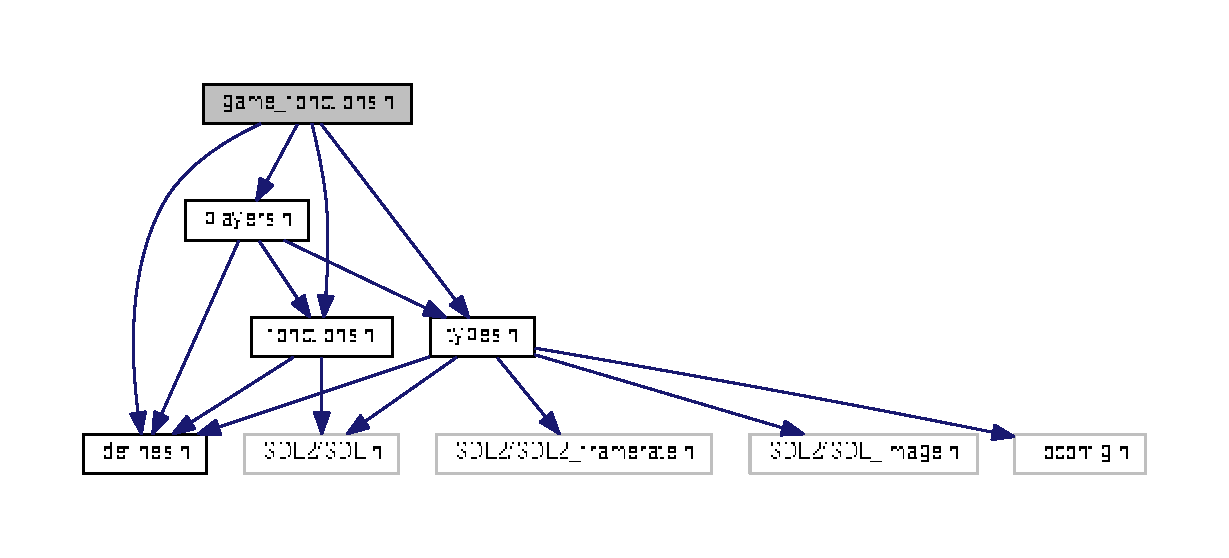
\includegraphics[width=350pt]{game__fonctions_8h__incl}
\end{center}
\end{figure}
Ce graphe montre quels fichiers incluent directement ou indirectement ce fichier \+:
\nopagebreak
\begin{figure}[H]
\begin{center}
\leavevmode
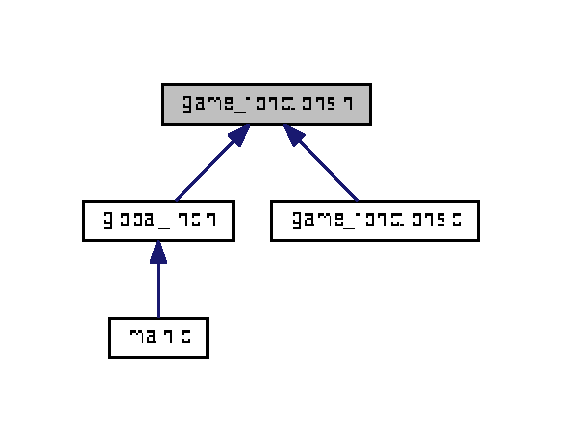
\includegraphics[width=270pt]{game__fonctions_8h__dep__incl}
\end{center}
\end{figure}
\subsection*{Fonctions}
\begin{DoxyCompactItemize}
\item 
\mbox{\label{game__fonctions_8h_ab3538182e6fae78c414c6b371c6f9b77}} 
void {\bfseries launch\+\_\+menu} (void)
\item 
\mbox{\label{game__fonctions_8h_ae1e52800cf2d4cb84e2c71d6af390622}} 
void {\bfseries launch\+\_\+game} (void)
\item 
\mbox{\label{game__fonctions_8h_af44b6382ab2dcccef07d61d735915bfa}} 
void {\bfseries launch\+\_\+replay} (void)
\item 
\mbox{\label{game__fonctions_8h_ae38078a115bc28d56f1e559a188e7437}} 
int {\bfseries init\+Window\+And\+Renderer} (S\+D\+L\+\_\+\+Window $\ast$$\ast$window, S\+D\+L\+\_\+\+Renderer $\ast$$\ast$renderer, const unsigned int width, const unsigned int height, const char $\ast$title)
\item 
\mbox{\label{game__fonctions_8h_a4dd7e919802a1f82dd6020412e5db80f}} 
int {\bfseries init\+S\+D\+L\+Systems} (F\+P\+Smanager $\ast$manager)
\item 
\mbox{\label{game__fonctions_8h_a5c9adc58626460dbf4f5280f43cafebf}} 
\textbf{ Game\+Data} $\ast$ {\bfseries create\+Game\+Data} (S\+D\+L\+\_\+\+Window $\ast$$\ast$window, S\+D\+L\+\_\+\+Renderer $\ast$$\ast$renderer, char $\ast$app\+Name)
\end{DoxyCompactItemize}


\subsection{Description détaillée}
Define the prototypes of core functions. 

\begin{DoxyAuthor}{Auteur}
Marius Monnier 
\end{DoxyAuthor}
\begin{DoxyVersion}{Version}
0.\+1 
\end{DoxyVersion}

\section{Référence du fichier global\+\_\+inc.\+h}
\label{global__inc_8h}\index{global\+\_\+inc.\+h@{global\+\_\+inc.\+h}}
{\ttfamily \#include $<$S\+D\+L2/\+S\+D\+L.\+h$>$}\newline
{\ttfamily \#include \char`\"{}S\+D\+L2/\+S\+D\+L2\+\_\+framerate.\+h\char`\"{}}\newline
{\ttfamily \#include $<$S\+D\+L2/\+S\+D\+L\+\_\+image.\+h$>$}\newline
{\ttfamily \#include $<$S\+D\+L2/\+S\+D\+L\+\_\+ttf.\+h$>$}\newline
{\ttfamily \#include $<$libconfig.\+h$>$}\newline
{\ttfamily \#include \char`\"{}defines.\+h\char`\"{}}\newline
{\ttfamily \#include \char`\"{}quit.\+h\char`\"{}}\newline
{\ttfamily \#include \char`\"{}fonctions.\+h\char`\"{}}\newline
{\ttfamily \#include \char`\"{}game\+\_\+fonctions.\+h\char`\"{}}\newline
{\ttfamily \#include \char`\"{}players.\+h\char`\"{}}\newline
Graphe des dépendances par inclusion de global\+\_\+inc.\+h\+:
\nopagebreak
\begin{figure}[H]
\begin{center}
\leavevmode
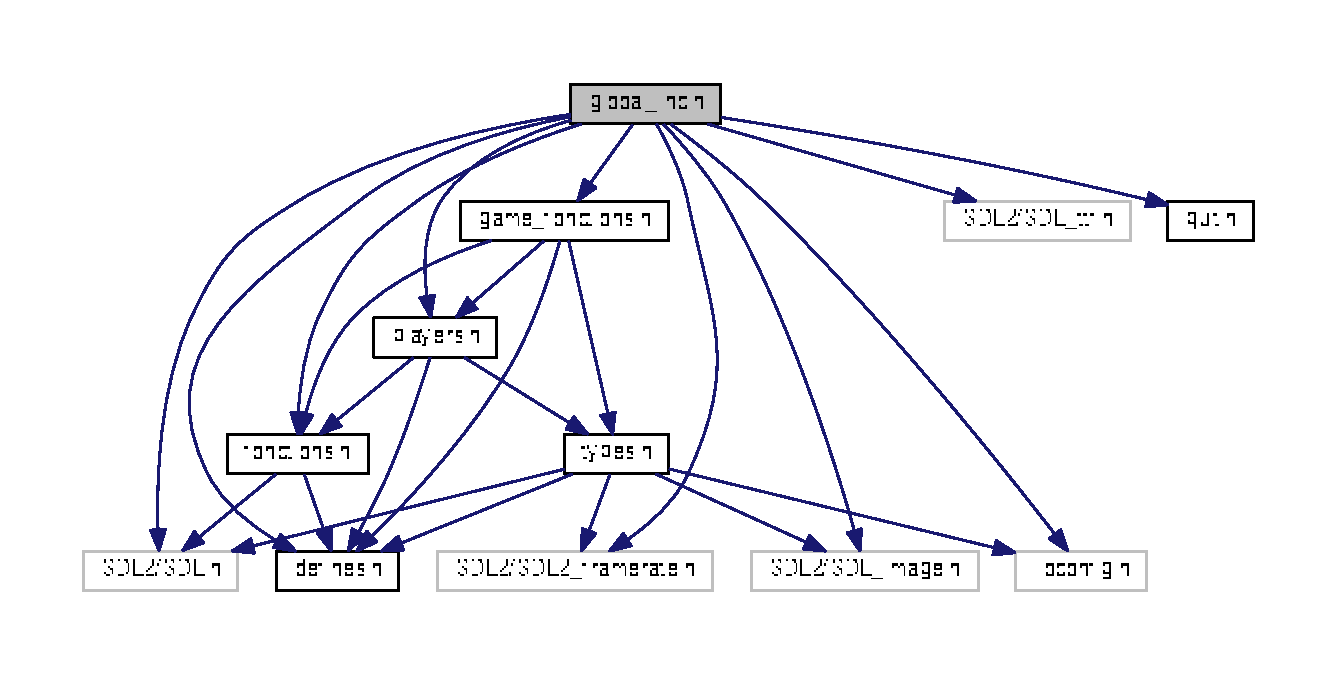
\includegraphics[width=350pt]{global__inc_8h__incl}
\end{center}
\end{figure}
Ce graphe montre quels fichiers incluent directement ou indirectement ce fichier \+:
\nopagebreak
\begin{figure}[H]
\begin{center}
\leavevmode
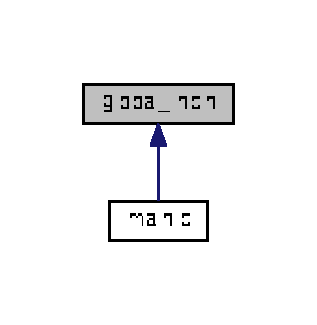
\includegraphics[width=152pt]{global__inc_8h__dep__incl}
\end{center}
\end{figure}


\subsection{Description détaillée}
Utility file for inclusion. 

\begin{DoxyAuthor}{Auteur}
Marius Monnier 
\end{DoxyAuthor}
\begin{DoxyVersion}{Version}
0.\+1 
\end{DoxyVersion}

\section{Référence du fichier main.\+c}
\label{main_8c}\index{main.\+c@{main.\+c}}
{\ttfamily \#include $<$stdlib.\+h$>$}\newline
{\ttfamily \#include $<$stdio.\+h$>$}\newline
{\ttfamily \#include \char`\"{}global\+\_\+inc.\+h\char`\"{}}\newline
Graphe des dépendances par inclusion de main.\+c\+:
\nopagebreak
\begin{figure}[H]
\begin{center}
\leavevmode
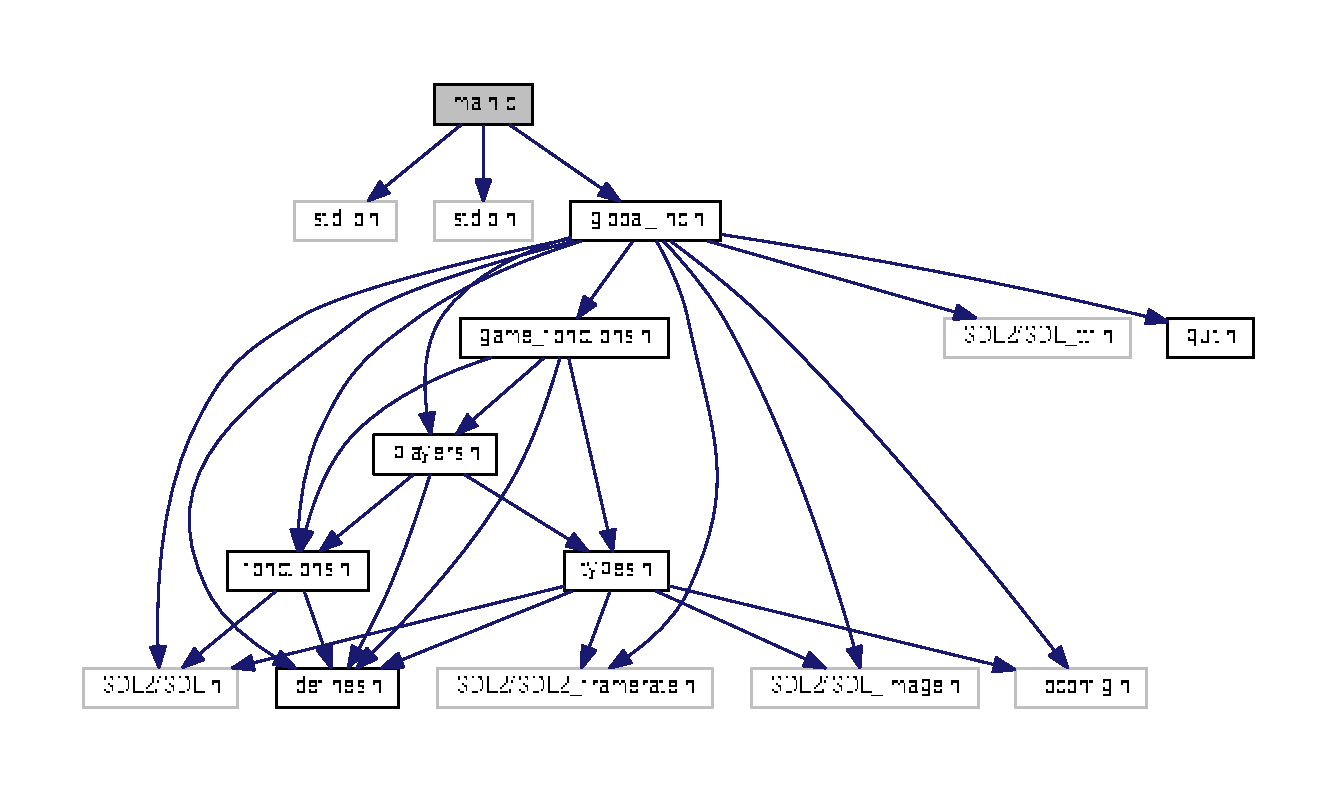
\includegraphics[width=350pt]{main_8c__incl}
\end{center}
\end{figure}
\subsection*{Fonctions}
\begin{DoxyCompactItemize}
\item 
\mbox{\label{main_8c_a840291bc02cba5474a4cb46a9b9566fe}} 
int {\bfseries main} (void)
\end{DoxyCompactItemize}
\subsection*{Variables}
\begin{DoxyCompactItemize}
\item 
\textbf{ Game\+Data} $\ast$ \textbf{ data} = N\+U\+LL
\item 
\mbox{\label{main_8c_a584a54ede29d504a2dc81d981781524c}} 
\textbf{ player} $\ast$ {\bfseries players} [\textbf{ M\+A\+X\+\_\+\+P\+L\+A\+Y\+E\+RS}]
\end{DoxyCompactItemize}


\subsection{Description détaillée}
Entry point of program. 

\begin{DoxyAuthor}{Auteur}
Marius Monnier 
\end{DoxyAuthor}
\begin{DoxyVersion}{Version}
0.\+1 
\end{DoxyVersion}


\subsection{Documentation des variables}
\mbox{\label{main_8c_a882ad77a7df764b098f98136eb56a83a}} 
\index{main.\+c@{main.\+c}!data@{data}}
\index{data@{data}!main.\+c@{main.\+c}}
\subsubsection{data}
{\footnotesize\ttfamily \textbf{ Game\+Data}$\ast$ data = N\+U\+LL}

$<$ Variable globale d\textquotesingle{}accès aux paramètres Tableau global des joueurs 

Définition à la ligne 12 du fichier main.\+c.


\section{Référence du fichier players.\+c}
\label{players_8c}\index{players.\+c@{players.\+c}}
{\ttfamily \#include \char`\"{}players.\+h\char`\"{}}\newline
Graphe des dépendances par inclusion de players.\+c\+:
\nopagebreak
\begin{figure}[H]
\begin{center}
\leavevmode
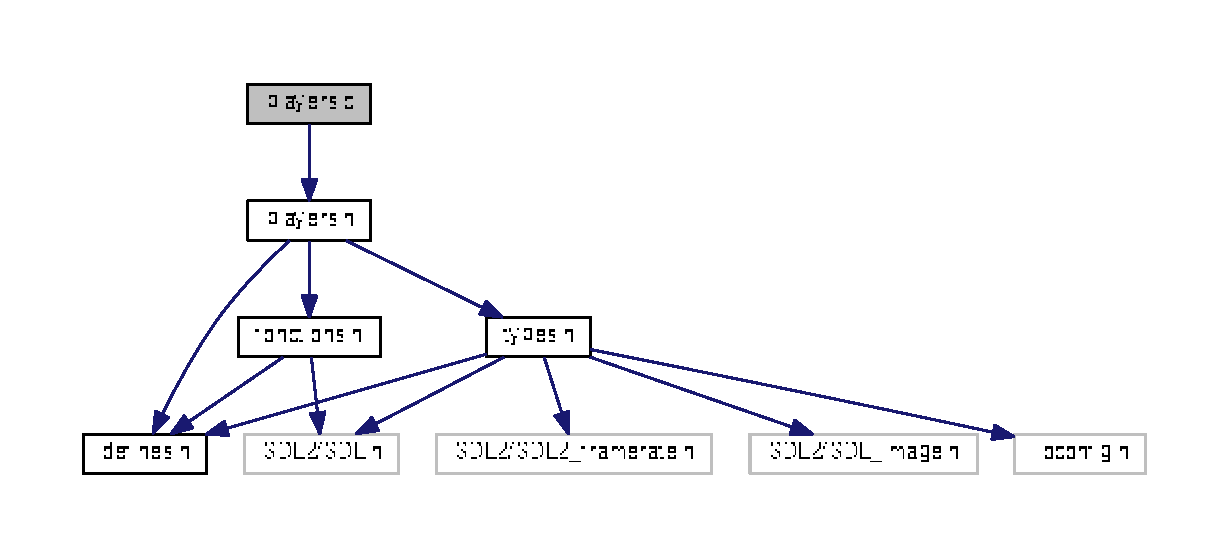
\includegraphics[width=350pt]{players_8c__incl}
\end{center}
\end{figure}
\subsection*{Fonctions}
\begin{DoxyCompactItemize}
\item 
\mbox{\label{players_8c_a171ccb671f0ad6a46718654fa0bffe10}} 
void {\bfseries set\+DirectionX} (\textbf{ player} $\ast$p, const \textbf{ Direction} dx)
\item 
\mbox{\label{players_8c_a63a649863120589ee459cf7a08902f95}} 
void {\bfseries set\+DirectionY} (\textbf{ player} $\ast$p, const \textbf{ Direction} dy)
\item 
\mbox{\label{players_8c_a84c122fe1272a6e56f76ea5597697bbe}} 
void {\bfseries set\+Direction} (\textbf{ player} $\ast$p, const \textbf{ Direction} dx, const \textbf{ Direction} dy)
\item 
\mbox{\label{players_8c_a8ceebefb9c41af5ee039bd4df9119f92}} 
int {\bfseries delete\+Player} (\textbf{ player} $\ast$play)
\item 
\mbox{\label{players_8c_abca54efb4fd2424881e91bcd7da8061a}} 
void {\bfseries set\+Score} (\textbf{ player} $\ast$p, double score)
\item 
\mbox{\label{players_8c_a252268c4afe2b752fd8b66f9c96a8df0}} 
void {\bfseries set\+Speed} (\textbf{ player} $\ast$p, \textbf{ Speed} sx, \textbf{ Speed} sy)
\item 
\textbf{ player} $\ast$ \textbf{ create\+Player} ()
\item 
\mbox{\label{players_8c_ae755369dabeb0a70730fbefb1d2d0972}} 
void {\bfseries move\+Player} (\textbf{ player} $\ast$p)
\item 
\mbox{\label{players_8c_a8bdc5cc263575cf5cf97c08e8d596293}} 
int {\bfseries delete\+All\+Players} ()
\end{DoxyCompactItemize}
\subsection*{Variables}
\begin{DoxyCompactItemize}
\item 
\textbf{ Game\+Data} $\ast$ \textbf{ data}
\item 
\mbox{\label{players_8c_aa6e0d10ac9dacf902c351a3cbb8a474d}} 
\textbf{ player} $\ast$ {\bfseries players} [$\,$]
\end{DoxyCompactItemize}


\subsection{Description détaillée}
Implement public players related functions and static painters related functions. 

\begin{DoxyAuthor}{Auteur}
Marius Monnier 
\end{DoxyAuthor}
\begin{DoxyVersion}{Version}
0.\+1 
\end{DoxyVersion}


\subsection{Documentation des fonctions}
\mbox{\label{players_8c_a232779641e812885a1fbc89b620b4848}} 
\index{players.\+c@{players.\+c}!create\+Player@{create\+Player}}
\index{create\+Player@{create\+Player}!players.\+c@{players.\+c}}
\subsubsection{create\+Player()}
{\footnotesize\ttfamily \textbf{ player}$\ast$ create\+Player (\begin{DoxyParamCaption}{ }\end{DoxyParamCaption})}



Function that create a player in interaction with user. 

\begin{DoxyReturn}{Renvoie}
A pointer to the created player if success, N\+U\+LL otherwise.
\end{DoxyReturn}
\begin{DoxyRefDesc}{A faire}
\item[\textbf{ A faire}]Change the way to preconfigured players. \end{DoxyRefDesc}


Définition à la ligne 240 du fichier players.\+c.



\subsection{Documentation des variables}
\mbox{\label{players_8c_a882ad77a7df764b098f98136eb56a83a}} 
\index{players.\+c@{players.\+c}!data@{data}}
\index{data@{data}!players.\+c@{players.\+c}}
\subsubsection{data}
{\footnotesize\ttfamily \textbf{ Game\+Data}$\ast$ data}

$<$ Variable globale d\textquotesingle{}accès aux paramètres Tableau global des joueurs 

Définition à la ligne 12 du fichier main.\+c.


\section{Référence du fichier players.\+h}
\label{players_8h}\index{players.\+h@{players.\+h}}
{\ttfamily \#include \char`\"{}defines.\+h\char`\"{}}\newline
{\ttfamily \#include \char`\"{}fonctions.\+h\char`\"{}}\newline
{\ttfamily \#include \char`\"{}types.\+h\char`\"{}}\newline
Graphe des dépendances par inclusion de players.\+h\+:
\nopagebreak
\begin{figure}[H]
\begin{center}
\leavevmode
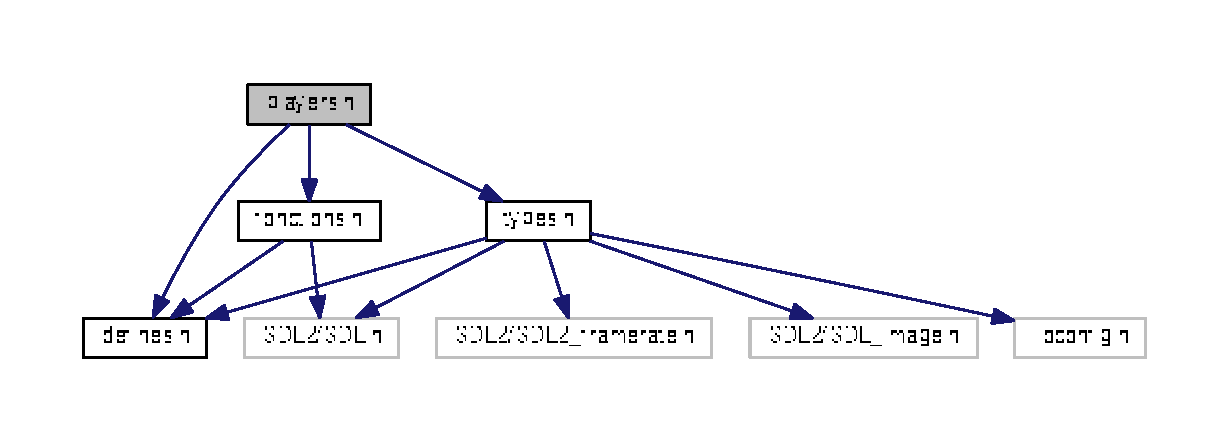
\includegraphics[width=350pt]{players_8h__incl}
\end{center}
\end{figure}
Ce graphe montre quels fichiers incluent directement ou indirectement ce fichier \+:
\nopagebreak
\begin{figure}[H]
\begin{center}
\leavevmode
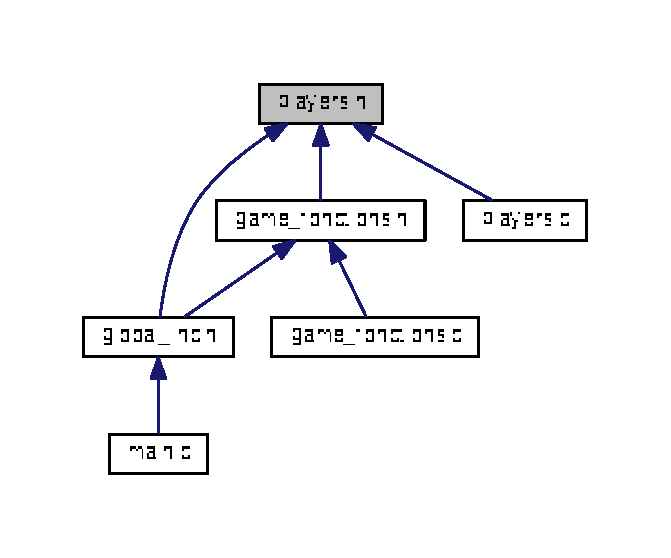
\includegraphics[width=322pt]{players_8h__dep__incl}
\end{center}
\end{figure}
\subsection*{Fonctions}
\begin{DoxyCompactItemize}
\item 
\textbf{ player} $\ast$ \textbf{ create\+Player} ()
\item 
\mbox{\label{players_8h_aee97302da473b6f7f4f27926d73abb3d}} 
void {\bfseries set\+DirectionX} (\textbf{ player} $\ast$, const \textbf{ Direction})
\item 
\mbox{\label{players_8h_a16ad2824483db11ccb9602acb5e1ac29}} 
void {\bfseries set\+DirectionY} (\textbf{ player} $\ast$, const \textbf{ Direction})
\item 
\mbox{\label{players_8h_a99eb8726cbcfd95c0634027792344069}} 
void {\bfseries set\+Direction} (\textbf{ player} $\ast$, const \textbf{ Direction}, const \textbf{ Direction})
\item 
\mbox{\label{players_8h_a26832b35489278e57f5fd92bfaf89216}} 
void {\bfseries move\+Player} (\textbf{ player} $\ast$)
\item 
\mbox{\label{players_8h_a8ceebefb9c41af5ee039bd4df9119f92}} 
int {\bfseries delete\+Player} (\textbf{ player} $\ast$play)
\item 
\mbox{\label{players_8h_a8bdc5cc263575cf5cf97c08e8d596293}} 
int {\bfseries delete\+All\+Players} ()
\end{DoxyCompactItemize}


\subsection{Description détaillée}
Define players related functions prototypes. 

\begin{DoxyAuthor}{Auteur}
Marius Monnier 
\end{DoxyAuthor}
\begin{DoxyVersion}{Version}
0.\+1 
\end{DoxyVersion}


\subsection{Documentation des fonctions}
\mbox{\label{players_8h_a62a16a32a68ba4359f95213cd4e39e85}} 
\index{players.\+h@{players.\+h}!create\+Player@{create\+Player}}
\index{create\+Player@{create\+Player}!players.\+h@{players.\+h}}
\subsubsection{create\+Player()}
{\footnotesize\ttfamily \textbf{ player} $\ast$ create\+Player (\begin{DoxyParamCaption}{ }\end{DoxyParamCaption})}



Function that create a player in interaction with user. 

\begin{DoxyReturn}{Renvoie}
A pointer to the created player if success, N\+U\+LL otherwise.
\end{DoxyReturn}
\begin{DoxyRefDesc}{A faire}
\item[\textbf{ A faire}]Change the way to preconfigured players. \end{DoxyRefDesc}


Définition à la ligne 240 du fichier players.\+c.


\section{Référence du fichier quit.\+c}
\label{quit_8c}\index{quit.\+c@{quit.\+c}}
{\ttfamily \#include \char`\"{}S\+D\+L2/\+S\+D\+L.\+h\char`\"{}}\newline
{\ttfamily \#include \char`\"{}S\+D\+L2/\+S\+D\+L\+\_\+image.\+h\char`\"{}}\newline
{\ttfamily \#include \char`\"{}quit.\+h\char`\"{}}\newline
Graphe des dépendances par inclusion de quit.\+c\+:
\nopagebreak
\begin{figure}[H]
\begin{center}
\leavevmode
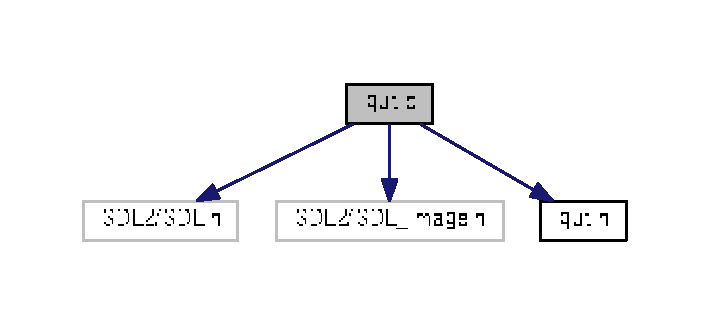
\includegraphics[width=341pt]{quit_8c__incl}
\end{center}
\end{figure}
\subsection*{Fonctions}
\begin{DoxyCompactItemize}
\item 
\mbox{\label{quit_8c_a041c01db677559185eea53ef91f60d1a}} 
void {\bfseries quit\+\_\+lib\+\_\+systems} ()
\end{DoxyCompactItemize}


\subsection{Description détaillée}
Define functions used at exit. 

\begin{DoxyAuthor}{Auteur}
Marius Monnier 
\end{DoxyAuthor}
\begin{DoxyVersion}{Version}
0.\+1 
\end{DoxyVersion}

\section{Référence du fichier quit.\+h}
\label{quit_8h}\index{quit.\+h@{quit.\+h}}
Ce graphe montre quels fichiers incluent directement ou indirectement ce fichier \+:
\nopagebreak
\begin{figure}[H]
\begin{center}
\leavevmode
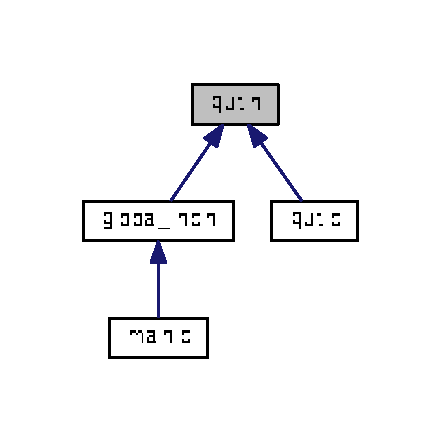
\includegraphics[width=212pt]{quit_8h__dep__incl}
\end{center}
\end{figure}
\subsection*{Fonctions}
\begin{DoxyCompactItemize}
\item 
\mbox{\label{quit_8h_a041c01db677559185eea53ef91f60d1a}} 
void {\bfseries quit\+\_\+lib\+\_\+systems} ()
\end{DoxyCompactItemize}


\subsection{Description détaillée}
Prototypes of exit functions. 

\begin{DoxyAuthor}{Auteur}
Marius Monnier 
\end{DoxyAuthor}
\begin{DoxyVersion}{Version}
0.\+1 
\end{DoxyVersion}

\section{Référence du fichier types.\+h}
\label{types_8h}\index{types.\+h@{types.\+h}}
{\ttfamily \#include \char`\"{}defines.\+h\char`\"{}}\newline
{\ttfamily \#include $<$S\+D\+L2/\+S\+D\+L.\+h$>$}\newline
{\ttfamily \#include \char`\"{}S\+D\+L2/\+S\+D\+L2\+\_\+framerate.\+h\char`\"{}}\newline
{\ttfamily \#include $<$S\+D\+L2/\+S\+D\+L\+\_\+image.\+h$>$}\newline
{\ttfamily \#include $<$libconfig.\+h$>$}\newline
Graphe des dépendances par inclusion de types.\+h\+:
\nopagebreak
\begin{figure}[H]
\begin{center}
\leavevmode
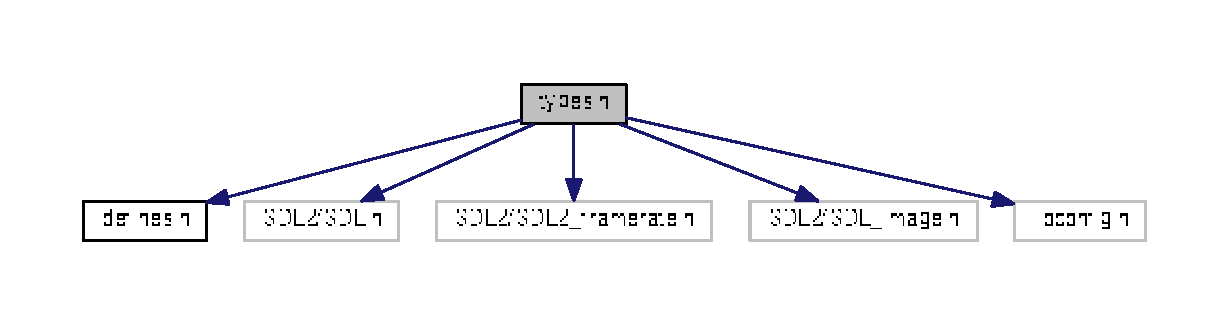
\includegraphics[width=350pt]{types_8h__incl}
\end{center}
\end{figure}
Ce graphe montre quels fichiers incluent directement ou indirectement ce fichier \+:
\nopagebreak
\begin{figure}[H]
\begin{center}
\leavevmode
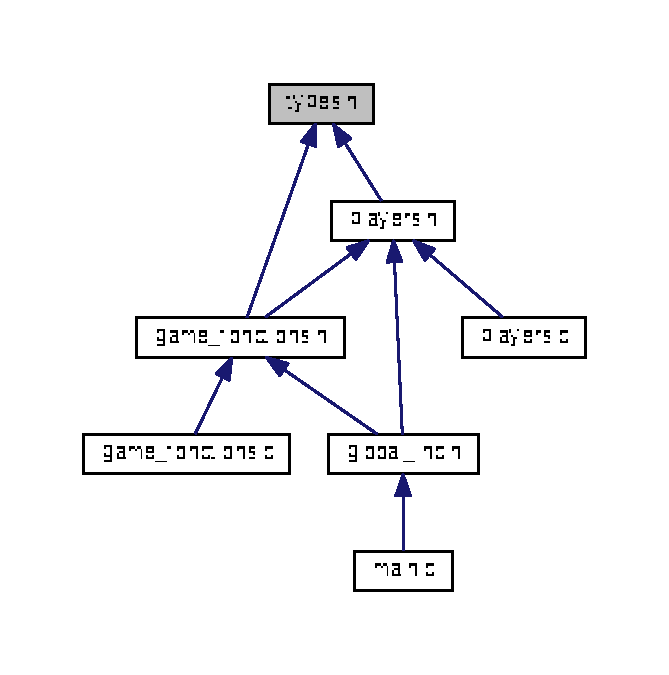
\includegraphics[width=321pt]{types_8h__dep__incl}
\end{center}
\end{figure}
\subsection*{Structures de données}
\begin{DoxyCompactItemize}
\item 
struct \textbf{ Direction\+Vector}
\item 
struct \textbf{ Speed\+Vector}
\item 
struct \textbf{ Screen}
\item 
struct \textbf{ Game\+Data}
\item 
struct \textbf{ painter}
\item 
struct \textbf{ player}
\end{DoxyCompactItemize}
\subsection*{Énumérations}
\begin{DoxyCompactItemize}
\item 
enum \textbf{ Direction} \{ \textbf{ D\+I\+R\+\_\+\+S\+T\+OP} =0, 
\textbf{ D\+I\+R\+\_\+\+A\+C\+T\+I\+VE} =1, 
\textbf{ D\+I\+R\+\_\+\+R\+E\+V\+E\+R\+SE} =-\/1
 \}
\item 
enum \textbf{ Brush\+Size} \{ \textbf{ B\+R\+U\+S\+H\+\_\+\+L\+I\+T\+T\+LE} =16, 
\textbf{ B\+R\+U\+S\+H\+\_\+\+N\+O\+R\+M\+AL} =32, 
\textbf{ B\+R\+U\+S\+H\+\_\+\+B\+IG} =64
 \}
\item 
enum \textbf{ Speed} \{ \textbf{ S\+P\+E\+E\+D\+\_\+\+N\+U\+LL} =0, 
\textbf{ S\+P\+E\+E\+D\+\_\+\+S\+L\+OW} =2, 
\textbf{ S\+P\+E\+E\+D\+\_\+\+A\+V\+E\+R\+A\+GE} =4, 
\textbf{ S\+P\+E\+E\+D\+\_\+\+F\+A\+ST} =6
 \}
\item 
enum \textbf{ Game\+State} \{ \textbf{ S\+T\+A\+T\+E\+\_\+\+Q\+U\+IT}, 
\textbf{ S\+T\+A\+T\+E\+\_\+\+P\+A\+U\+S\+ED}, 
\textbf{ S\+T\+A\+T\+E\+\_\+\+P\+L\+A\+Y\+I\+NG}, 
\textbf{ S\+T\+A\+T\+E\+\_\+\+C\+O\+N\+F\+I\+G\+U\+R\+A\+T\+I\+ON}
 \}
\item 
enum \textbf{ Control\+Keys} \{ \textbf{ C\+T\+R\+L\+\_\+\+K\+E\+Y\+\_\+\+R\+I\+G\+HT} =0, 
\textbf{ C\+T\+R\+L\+\_\+\+K\+E\+Y\+\_\+\+L\+E\+FT} =1, 
\textbf{ C\+T\+R\+L\+\_\+\+K\+E\+Y\+\_\+\+UP} =2, 
\textbf{ C\+T\+R\+L\+\_\+\+K\+E\+Y\+\_\+\+D\+O\+WN} =3
 \}
\end{DoxyCompactItemize}


\subsection{Description détaillée}
Types needed in program. 

\begin{DoxyAuthor}{Auteur}
Marius Monnier 
\end{DoxyAuthor}
\begin{DoxyVersion}{Version}
0.\+1 
\end{DoxyVersion}

%--- End generated contents ---

% Index
\backmatter
\newpage
\phantomsection
\clearemptydoublepage
\addcontentsline{toc}{chapter}{Index}
\printindex

\end{document}
